% !TEX encoding = UTF-8 Unicode
\documentclass{article}
\usepackage{geometry} % 設定邊界
\geometry{
  top=2in,
  inner=1in,
  outer=1in,
  bottom=1in,
  headheight=3ex,
  headsep=2ex
}

\usepackage{fontspec}   %加這個就可以設定字體
\usepackage{xeCJK}       %讓中英文字體分開設置
\setCJKmainfont{BiauKai} %設定中文為系統上的字型,而英文不去更動,使用原TeX字型
\setmainfont{Times} % 設定英文字型
\XeTeXlinebreaklocale "zh"             %這兩行一定要加,中文才能自動換行
\XeTeXlinebreakskip = 0pt plus 1pt     %這兩行一定要加,中文才能自動換行

\usepackage{titling}
\setlength{\droptitle}{-12em} % 將標題移動至頁面的上面


\title{第三章 - Python與Jupyter Notebook /線段偵測/道路判斷與車體控制}

\author{呂承龍}
\date{} %不要日期

\begin{document}
\maketitle

\section{Python與Jupyter Notebook}
\subsection{Python介紹}
Python是現在非常廣用的程式語言之一,相對於其他程式語言而言,它具有較易上手且較易閱讀的特徵。Python語言特別強調其可讀性,讓程式碼可以輕易地被他人理解。
\\另外,Python與C C++ Java等語言很不同的一點是,Python是一種直譯式的語言,意思是不需要先編譯(Compile)在執行,而是邊執行邊編譯。目前,Python也被廣泛地使用在資料科學裡面。

\subsection{Jupyter Notebook介紹}
Jupyter Notebook是一個網路應用程式,可以在裡面書寫程式碼並在網路上做分享。對於我們而言,他最方便的地方在於能將程式碼分成一個一個的區塊(Cell),並且分別觀看每個區塊的輸出結果。因為這樣的分辨性,讓我們可以分別檢查每段的程式,是否有期望中的輸出抑或是挑出其中的Bug。
\\不過要注意的是,Jupyter Notebook只能使用直譯式語言,例如python等等。在使用上要特別注意。

\subsection{小試身手!}
開啟Jupyter Notebook
\\接下來我們就來做一些練習,這裡會特別解釋Duckietown裡面會用到的部分。首先我們要先用Jupyter notebook打開練習用的檔案。
\\\$ duckietop@ cd ~/duckietown/tutorials/summer2017\_nctu/
\\\$ duckietop@ jupyter notebook 4-1.python\_tutorial.ipynb
\\\\快捷鍵教學
\\在快捷鍵的部分,我們按上下可以在不同的區間(cell)之間移動,按下Enter可以進入到cell裡面進行編輯,按下ESC可以離開。Shift+Enter一起按下就可以執行該區段的程式碼。按下a/b可以分別在該cell的上面或下面加一個新的cell,連按dd則可以刪除不需要的cell。1/2/3則可以分別加上不同粗細的註解。
\\以上就是常用的快捷鍵的部分,按下h就會重新顯示快捷鍵的列表,供大家使用。各位一定要自己試過,玩玩看,才會學得快喔!
\\\\Cell區間
\\我們來稍微解釋一下cell區間。請看下圖
\\每個區間都有一個程式碼的部分,請大家就把程式碼打在這裡。若該程式碼有輸出的話,下面則會顯示輸出的樣子。特別要注意的是旁邊的有一個In[],裡面可能有數字可能沒數字。數字代表的是執行的順序(如果有被執行的話)。因為程式碼之間順序是有差別的,若大家在還沒呼叫函式庫就先使用該函式庫的函式的話,就會出錯。
\\
\begin{figure}[htp]
    \begin{center}
        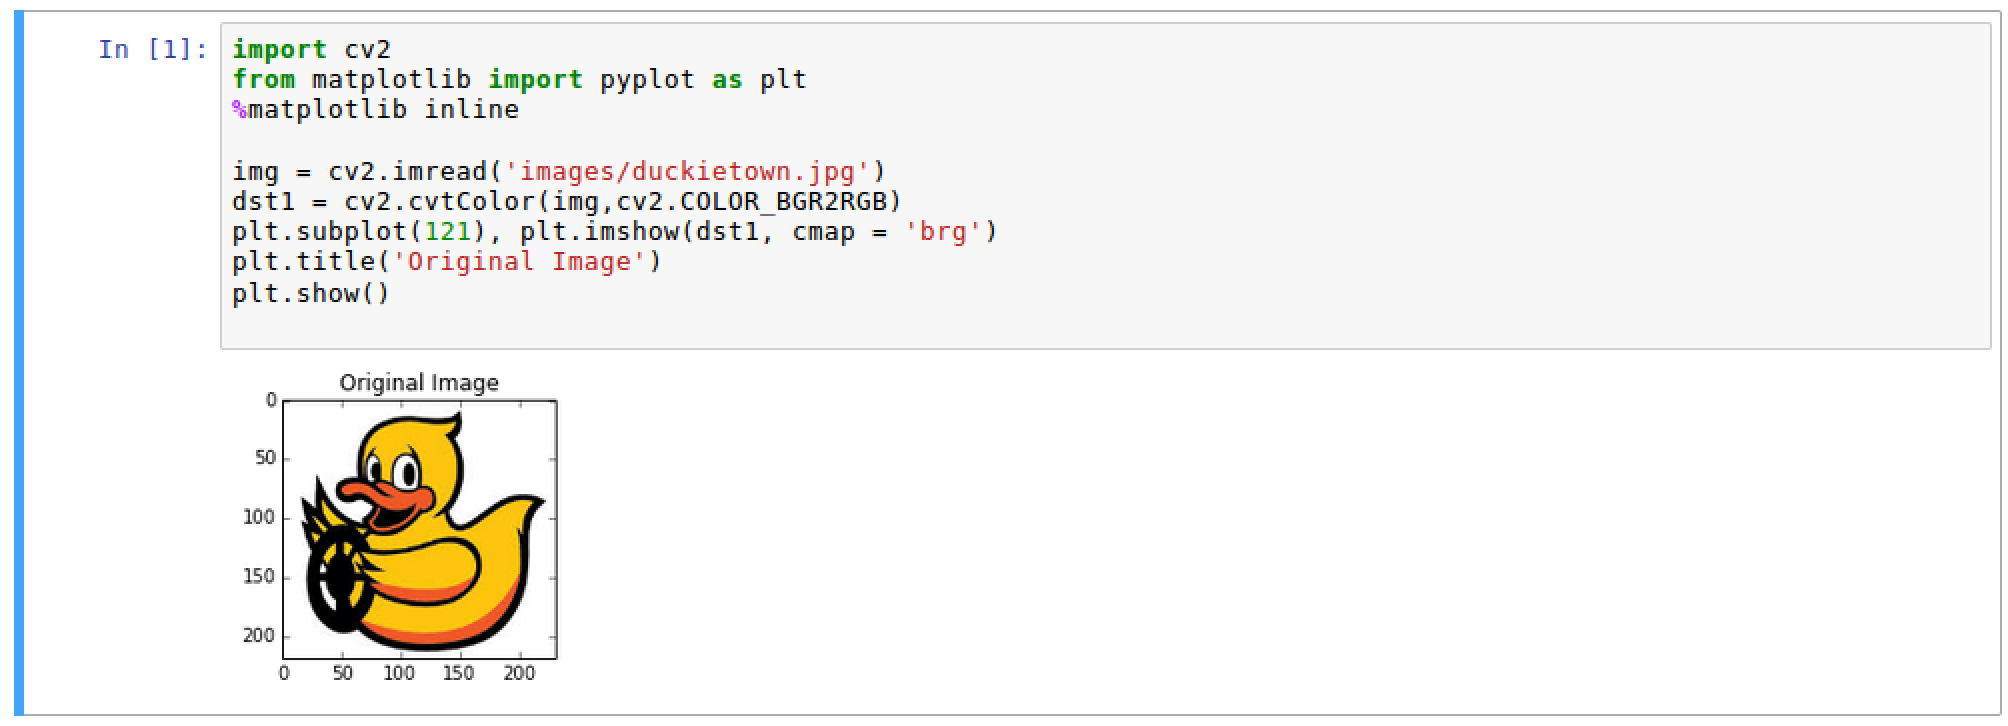
\includegraphics[width=450pt]{pic/3_1_1.png}
    \end{center}
\end{figure}
\\
\\\\\\\\\\\\基礎Python(print、迴圈、陣列)
\\開始要進入Python的部分了,首先我們先看print的部分,接下來的部分大家一定要自己動手玩玩看,調調裡面的參數,才會學得上手喔!
\\
\begin{figure}[htp]
    \begin{center}
        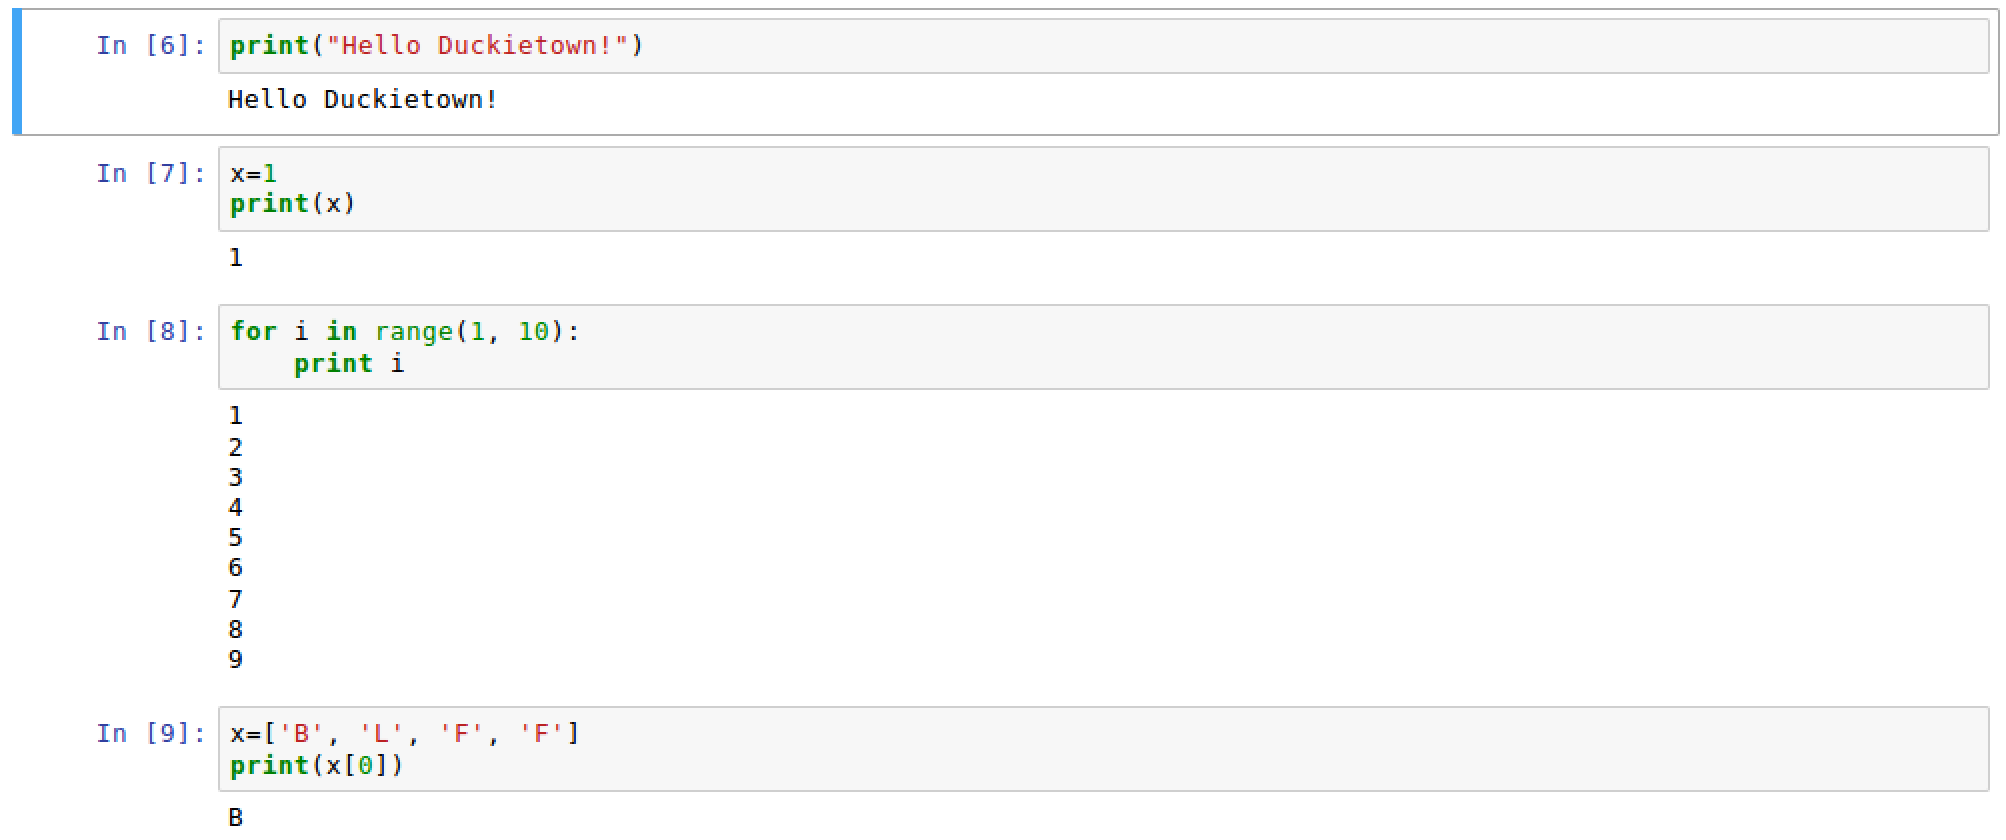
\includegraphics[width=450pt]{pic/3_1_2.png}
    \end{center}
\end{figure}
\\
\\首先我們可以發現到,python在參數宣告的部分很簡單,不需要特別宣告變數型態(例如:int, double等等),在print的地方也很簡單,只要直接將要輸入的變數放進去即可。如果要多個變數夾雜的話,可以用“,”隔開如下。
\\print x, ‘*’, x, ‘=’, x*x
\\另外再for迴圈的部分,會使用in range(n, m)來表達此迴圈的i要從n到m但不包含m。
\\再提醒一下各位,Python是一種不需要大括號的語言,也就是說他是靠縮排來表示不同部分,縮排可以用tab或是四個空白表示,但同一程式內只能用一種來當縮排喔!
\\接下來我們看一下陣列的部分
\\
\begin{figure}[htp]
    \begin{center}
        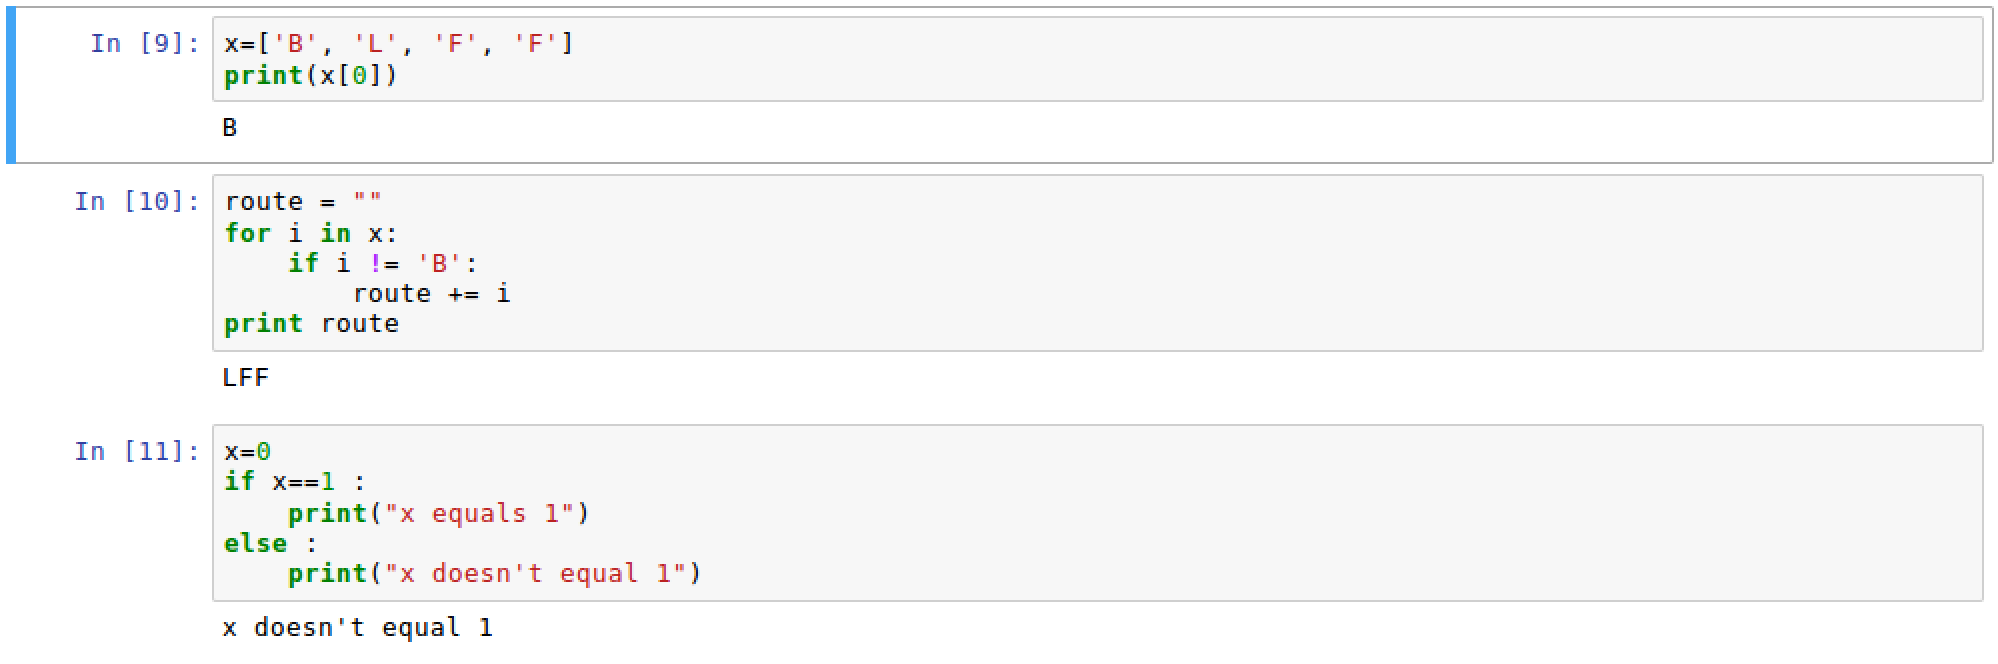
\includegraphics[width=450pt]{pic/3_1_3.png}
    \end{center}
\end{figure}
\\
我們可以看到,Python要宣告一個陣列也是非常簡單的,也可以結合for迴圈一起使用,大家可以自己試試看。
\\\\Numpy與Scipy
\\Numpy與Scipy是我們在分析與實驗常用到的兩個函式庫,我們一邊看圖一邊解釋
\\
\begin{figure}[htp]
    \begin{center}
        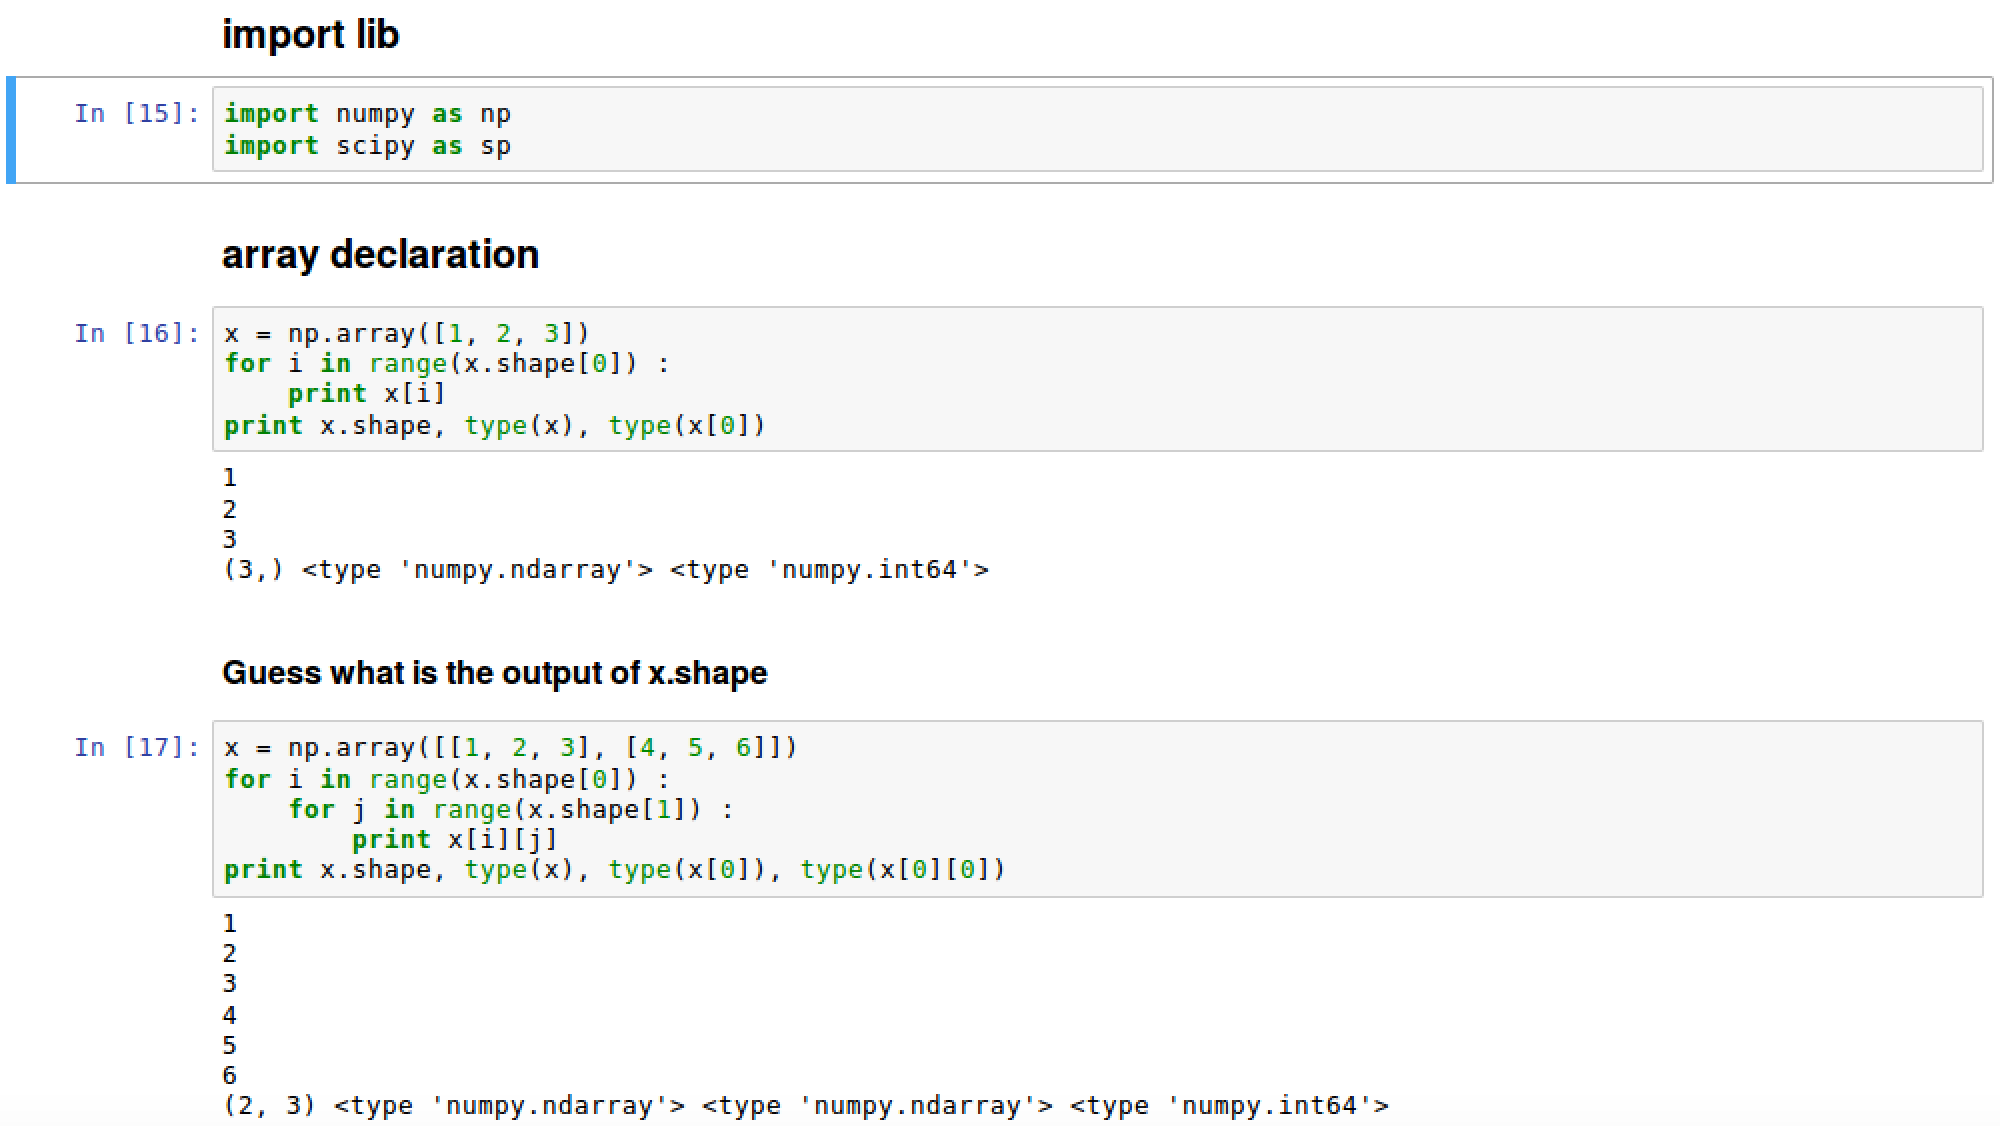
\includegraphics[width=450pt]{pic/3_1_5.png}
    \end{center}
\end{figure}
\\
我們要使用函式庫首先就要import他,後面的as np, as sp則是代表當我們之後要使用該函式庫的函式時,我們可以用np取代numpy,待會我們就會看到範例。
\\首先第一部分就是numpy的陣列,他的陣列夠強大,可以方便我們使用。
\\接著我們可以看到一個關鍵字x.shape,他的輸出會是x陣列個維度的大小,所以像是我們第一個cell的陣列只有一維、該維長度是3,所以x.shape輸出會是(3,)。下面一個cell就可以看到若有多維的陣列輸出會是什麼樣子。
\\至於type(),則可以輸出該資料的型態,裡面可以是變數,也可以是陣列等等。
\\
\begin{figure}[htp]
    \begin{center}
        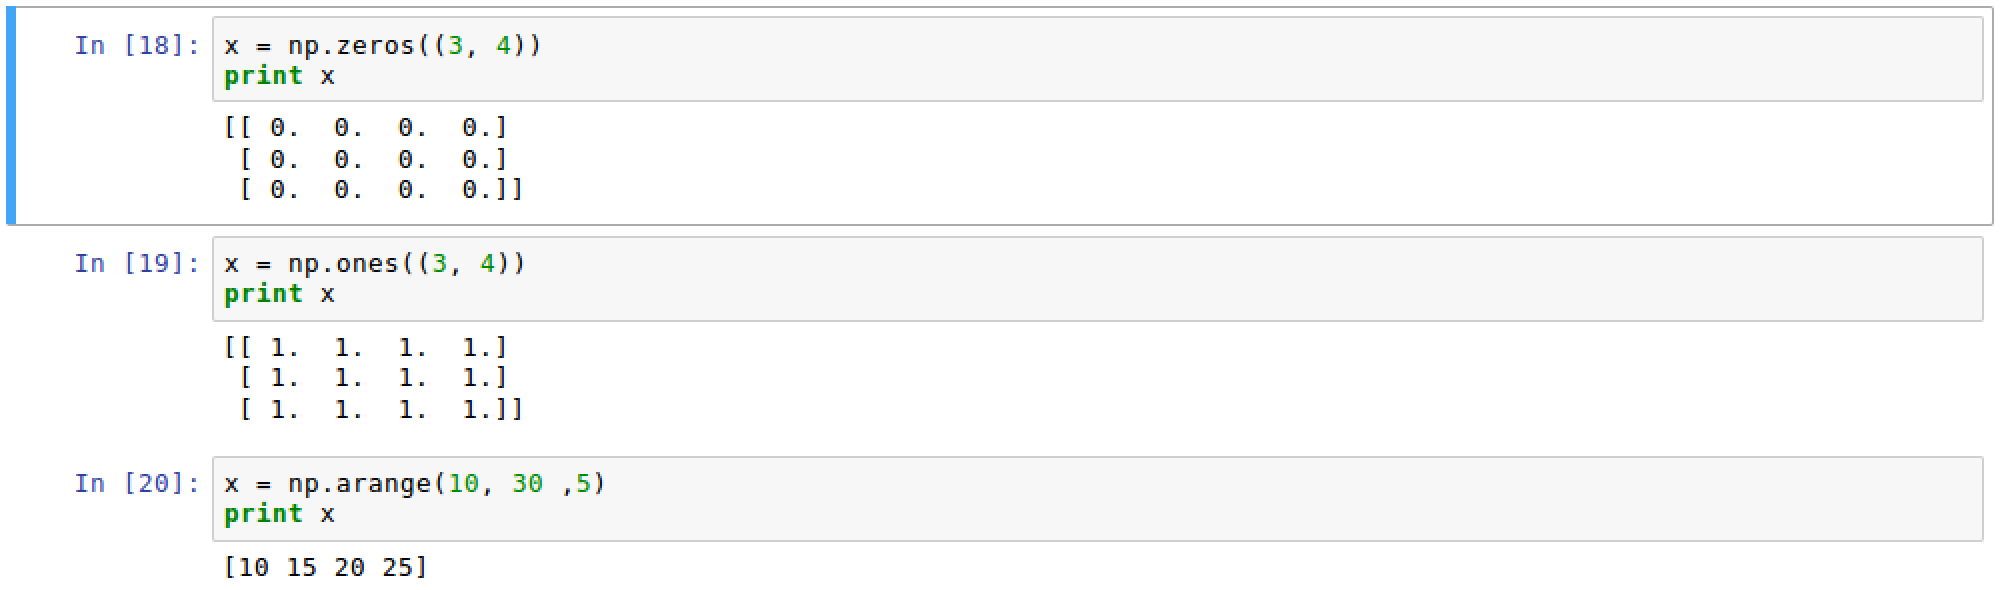
\includegraphics[width=450pt]{pic/3_1_6.png}
    \end{center}
\end{figure}
\\
而numpy也可以讓我們很快速產生一個零陣列或都是一的陣列。另外arange則是一個可以很方便產生固定距離數字陣列的函式,不過產生出來的東西只有一維的,如果我們要讓他變成多維的話,可以使用下面這種函式reshape。
\
\begin{figure}[htp]
    \begin{center}
        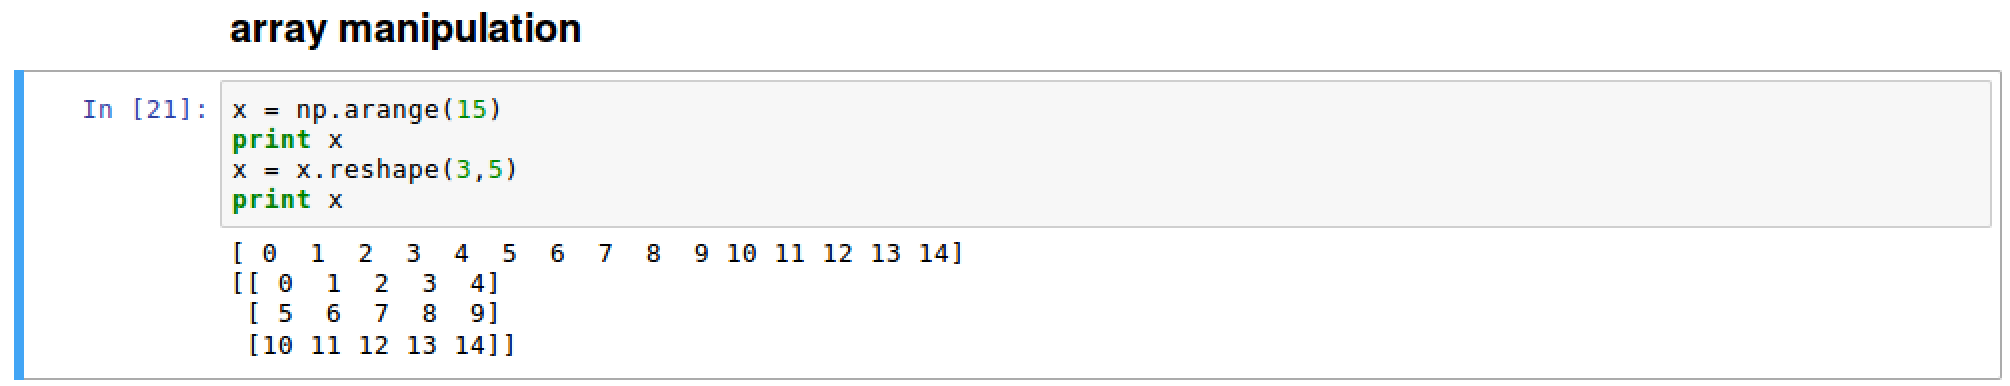
\includegraphics[width=450pt]{pic/3_1_7.png}
    \end{center}
\end{figure}
\\
用Python畫圖
\\我們在算數學的過程,常常會需要將其視覺化,接下來我們要介紹一種常用的函式庫,請看以下。
\\matplotlib是我們常用來畫圖的函式庫,我們會使用裡面的pyplot的
\
\begin{figure}[htp]
    \begin{center}
        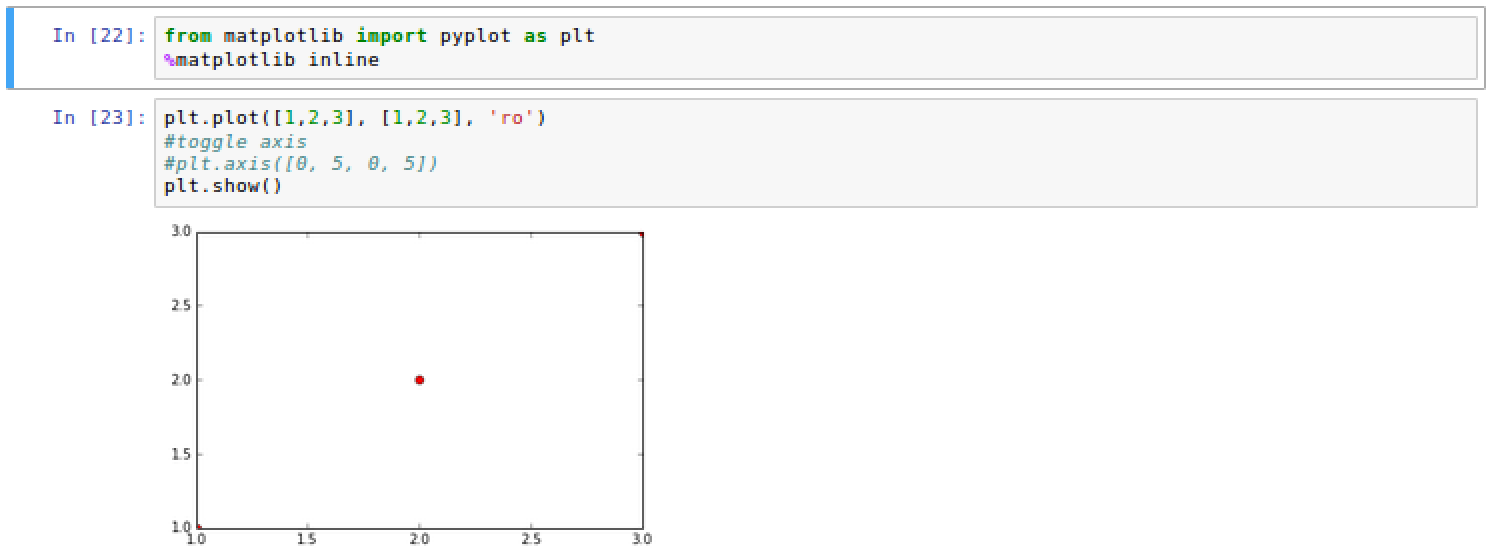
\includegraphics[width=450pt]{pic/3_1_8.png}
    \end{center}
\end{figure}
\\\\\\\\\\\\\\\\\\\\\\\\\\\\接下來這部分則是矩陣視覺化,有以顏色表示也有用單純的灰階來表示。
\\
\begin{figure}[htp]
    \begin{center}
        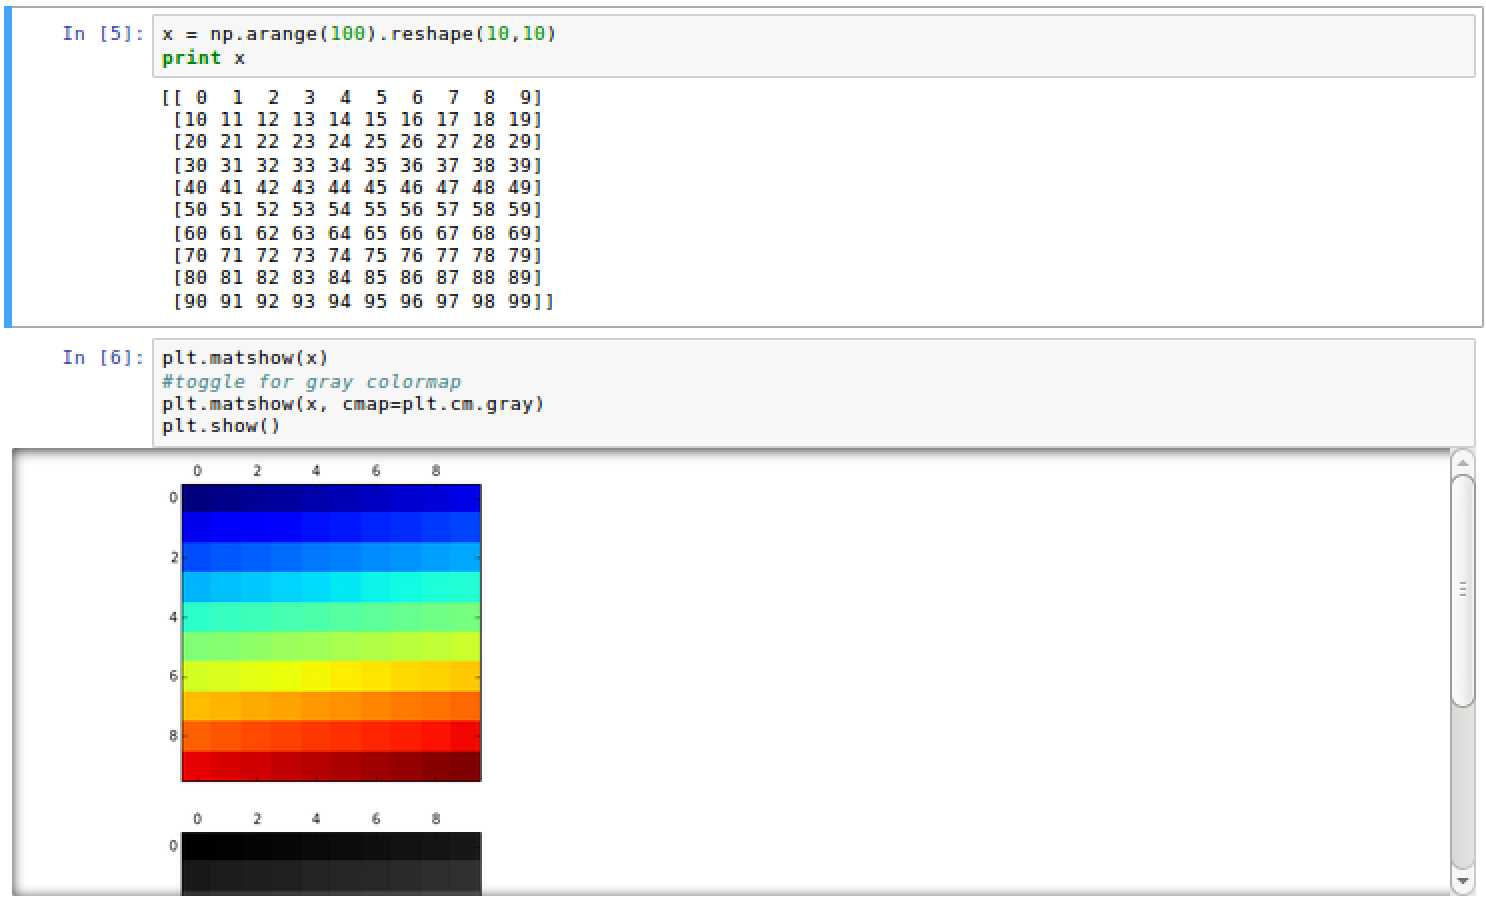
\includegraphics[width=400pt]{pic/3_1_9.png}
    \end{center}
\end{figure}
\\微積分與函數
\\剛剛有說明,numpy跟scipy都是很好用的工具,當然也可以拿來算微積分等等數學。
\begin{figure}[htp]
    \begin{center}
        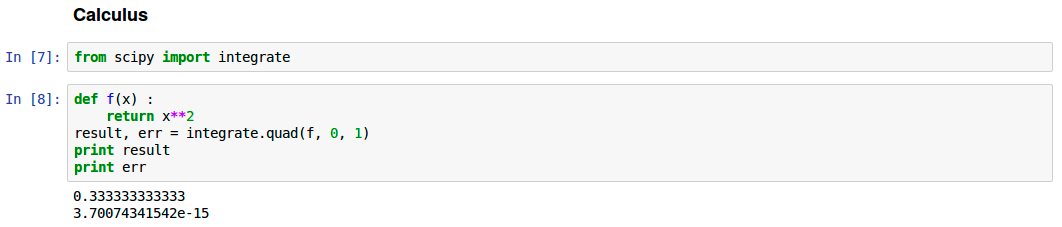
\includegraphics[width=400pt]{pic/3_1_10.png}
    \end{center}
\end{figure}
\\
在算數學時也常有把函數畫出圖來的動作,在numpy裡面也是做得到的喔!
\begin{figure}[htp]
    \begin{center}
        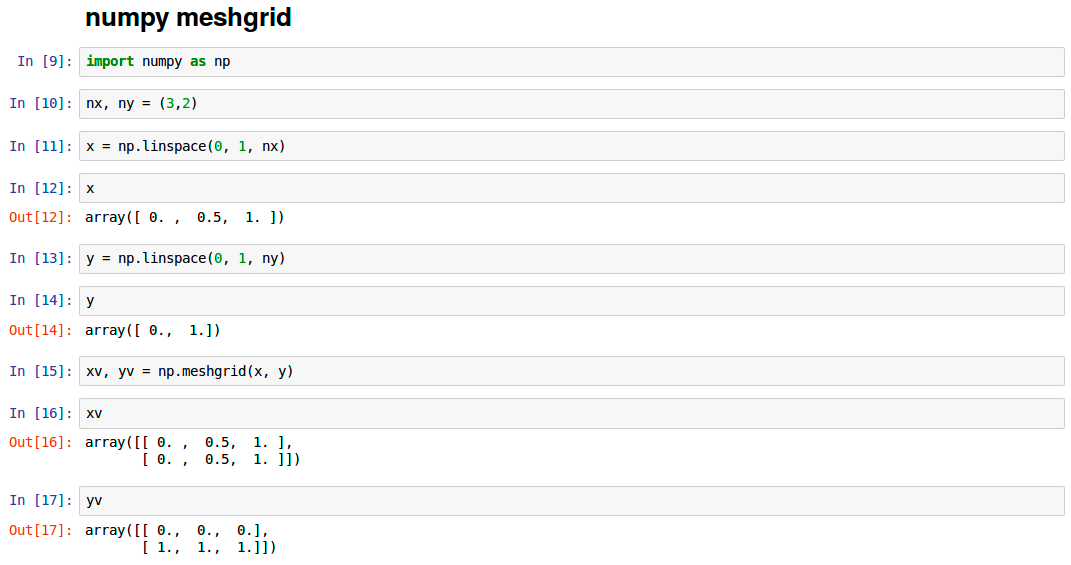
\includegraphics[width=400pt]{pic/3_1_11.png}
    \end{center}
\end{figure}
\\
對電腦來說,是沒有連續的東西,因此畫函數的第一步驟,是標出樣本點(Sample),這裡面所用的就是meshgrid函數。將自己需要的x, y座標點做出一個陣列,在丟進meshgrid函數,meshgrid會輸出兩個函數,待會分別拿來當x, y座標的樣本點。接下來要就是畫圖的部分,我們要畫的是z = sin(2x + 2y)/(2x + 2y)。一樣我們先meshgrid,接下來非常簡單,只要把丟進需要的函數就可以了,然後我們使用contourf來畫函數。
\begin{figure}[htp]
    \begin{center}
        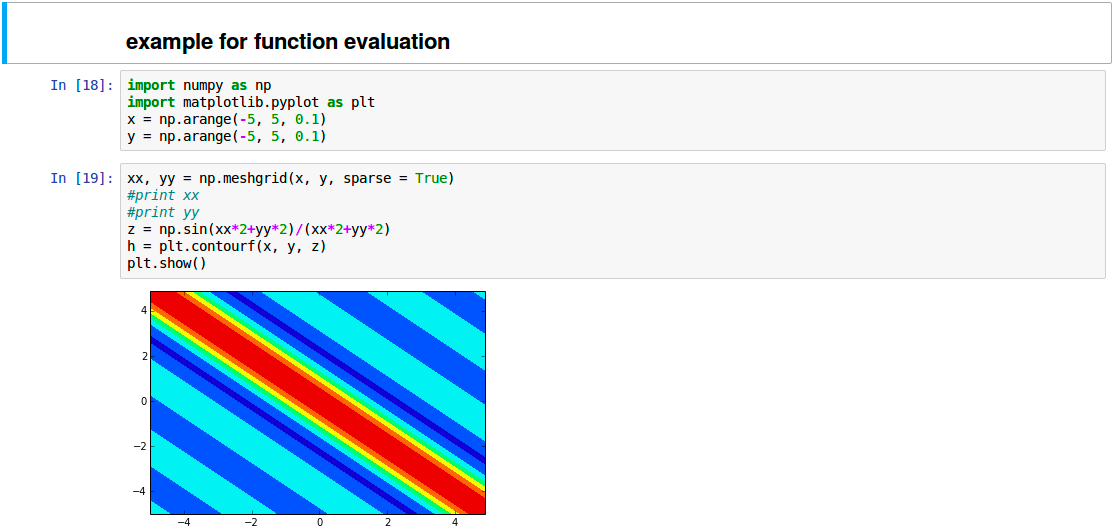
\includegraphics[width=400pt]{pic/3_1_12.png}
    \end{center}
\end{figure}
\\
牛刀小試
\\\\基本的Python以及Jupyter Notebook教學就到這邊囉!這邊有兩道小題目給大家做練習。
\\第一題:用for loop做出一個九九乘法表。
\
\begin{figure}[htp]
    \begin{center}
        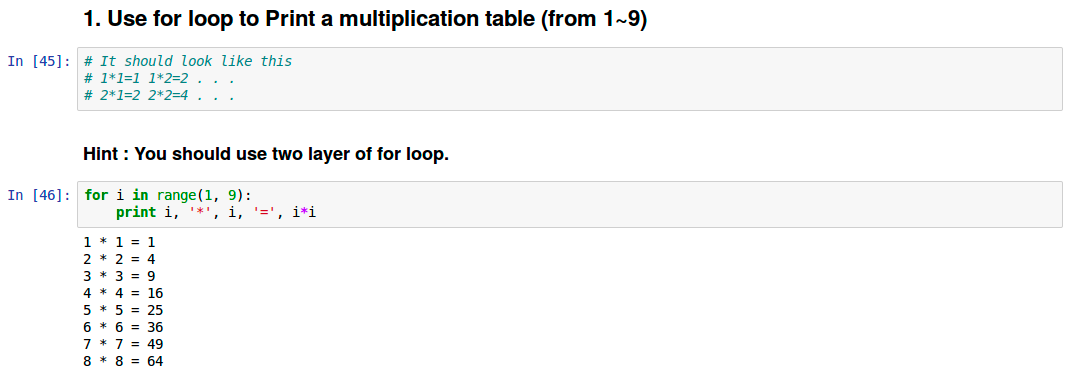
\includegraphics[width=400pt]{pic/3_1_13.png}
    \end{center}
\end{figure}
\\
第二題:畫出 z = cos(x\^2 + y\^2) 函數。
\
\begin{figure}[htp]
    \begin{center}
        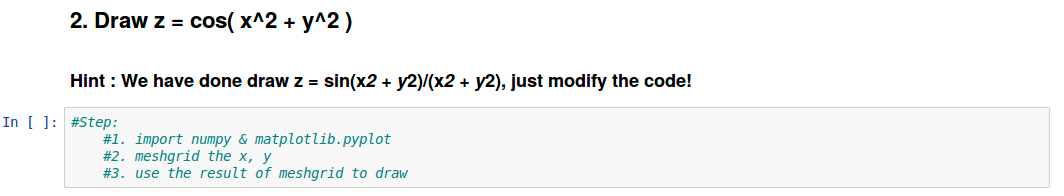
\includegraphics[width=400pt]{pic/3_1_14.png}
    \end{center}
\end{figure}
\\

\newpage
\section{線段偵測}
\subsection{自動駕駛流程圖}
這裡我們要先解釋一下在Duckietown裡自動駕駛的流程圖。
\
\begin{figure}[htp]
    \begin{center}
        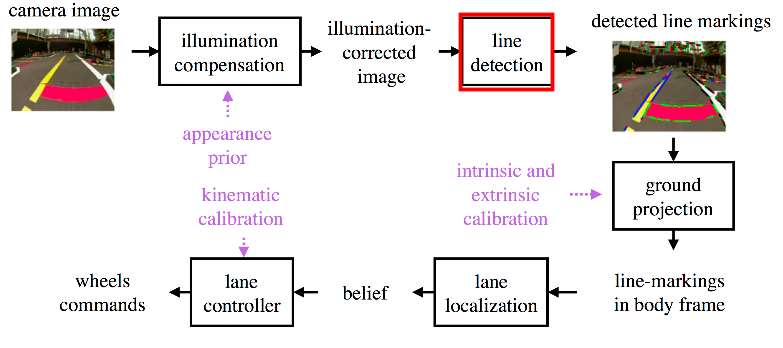
\includegraphics[width=450pt]{pic/3_2_1.png}
    \end{center}
\end{figure}
\\
在鏡頭得到圖片之後,這些圖會先利用程式調整光線對比,接著我們就會去偵測圖裡面的線段,也就是道路邊線的線段。接著偵測出來的光線會利用相機校正後得到的參數,得到每個線段在真實世界中的座標位置。接著利用這些線段判斷道路的位置以及車子的位置(專業用語是Pose”姿態”)。最後再給馬達做相對應的動力。

\subsection{線段偵測原理}
接著我們來解釋線段偵測的原理。
\
\begin{figure}[htp]
    \begin{center}
        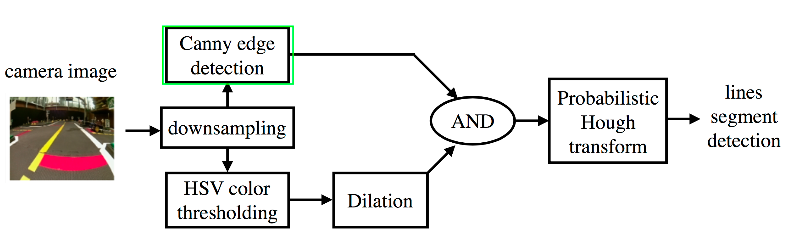
\includegraphics[width=450pt]{pic/3_2_2.png}
    \end{center}
\end{figure}
\\
首先會先縮小圖片以增加運算速度,接著圖片會分別經過Canny Edge Detector (Canny邊緣運算子)以及HSV Color Thresholding (HSV 顏色閾質判斷)。將兩邊所得的接過經過AND邏輯閘。最後再做Hough Transform (霍夫轉換)就可以得到結果了。

\subsection{Canny Edge Detector (Canny邊緣運算子)}
二維卷積
\\在解釋Canny Edge Detector之前我們先解釋偵測線斷的原理。一般而言,我們都是用Convolution (卷積)來判斷線段。我們先看下面的例子。
\begin{figure}[htp]
    \begin{center}
        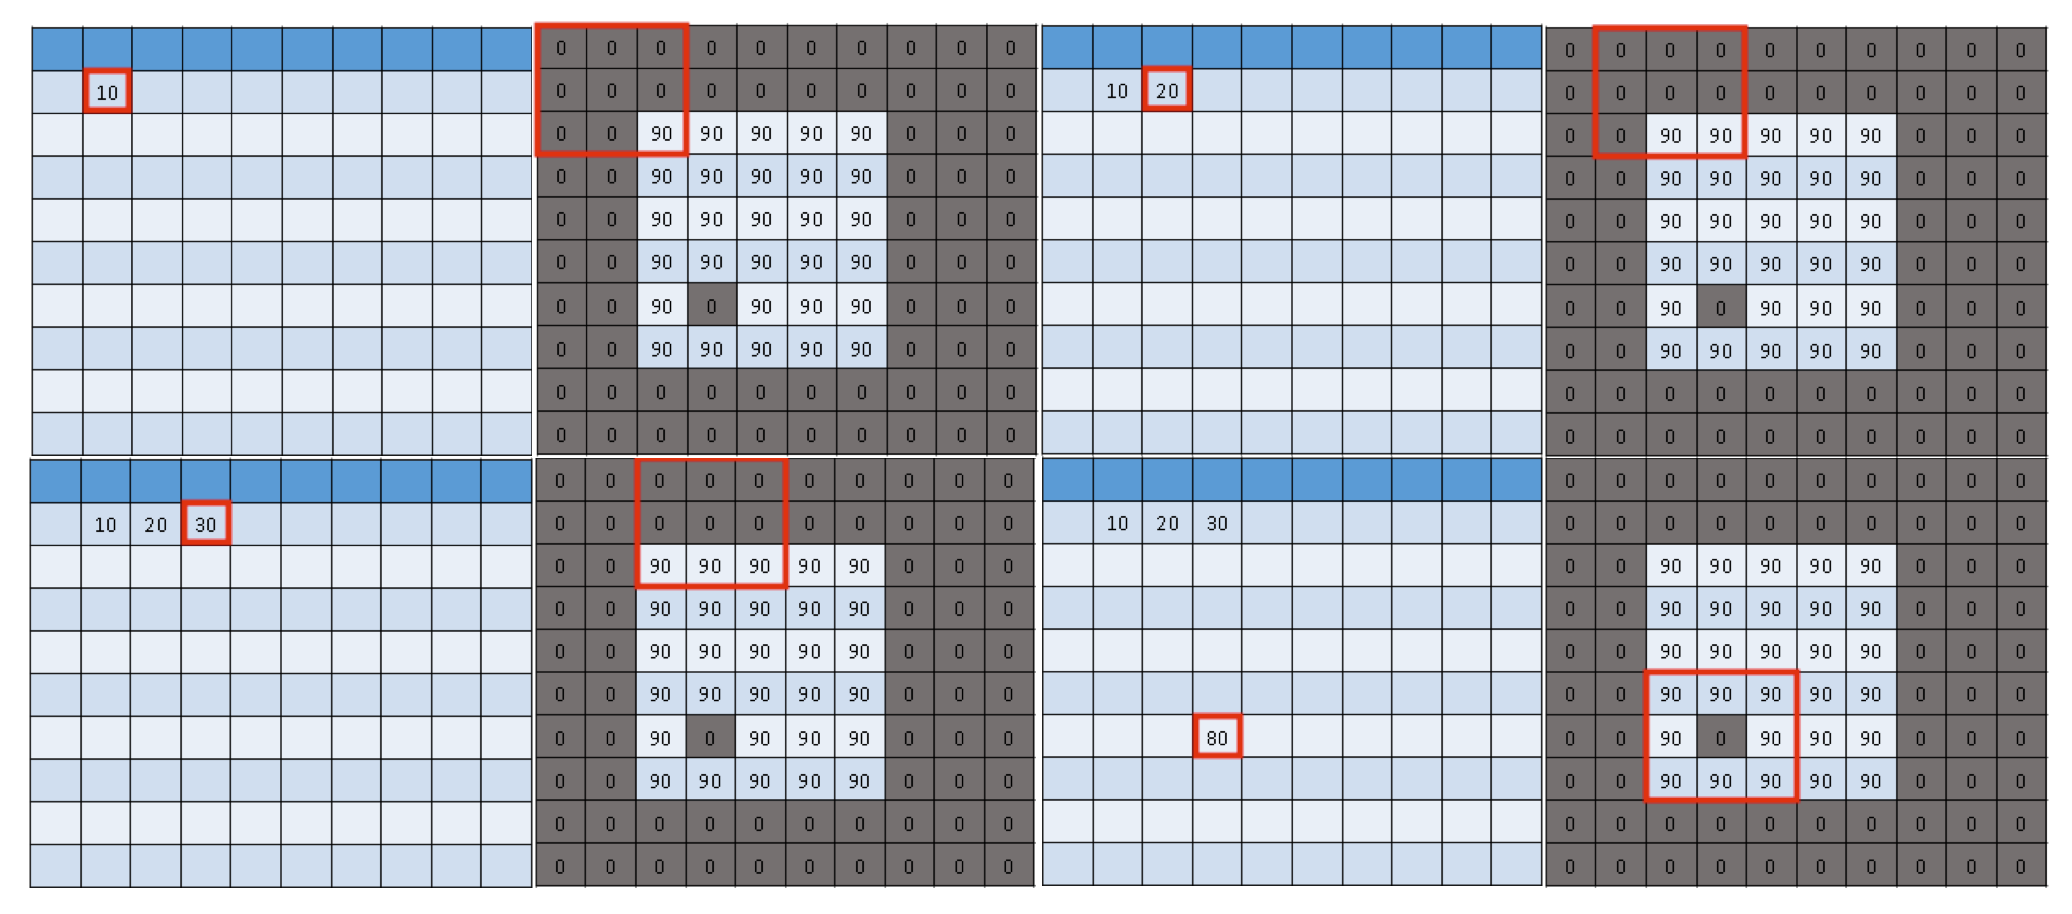
\includegraphics[width=450pt]{pic/3_2_3.png}
    \end{center}
\end{figure}
\\
先來解釋二維的卷積是怎麼運作的。基本上我們會把一個Kernel(紅色框框部分)與圖片中的像素點對齊,每個點乘以一之後,全部相加取平均,就是這個Kernel核心的那個像素點的值。接下來我們把Kernel不斷地向右移,就可以得到大部分像素點新的值。最後我們把最外圍的像素點補上0(有時候是補上最大值,看使用的地方而定)就大功告成了。
\begin{figure}[htp]
    \begin{center}
        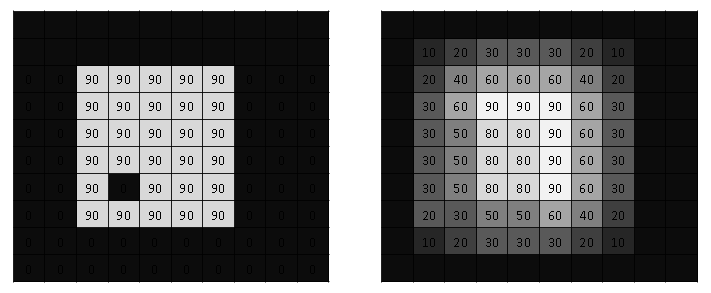
\includegraphics[width=300pt]{pic/3_2_4.png}
    \end{center}
\end{figure}
\\
Sobel Operator \& Canny Edge Detector
\\那麼二維卷積可以怎麼幫助我們呢?我們介紹一種Sobel Operator (索貝爾算子)。Sobel Filter基本上就是對圖片做二維卷積,但他的Kernel長這樣:
\begin{figure}[htp]
    \begin{center}
        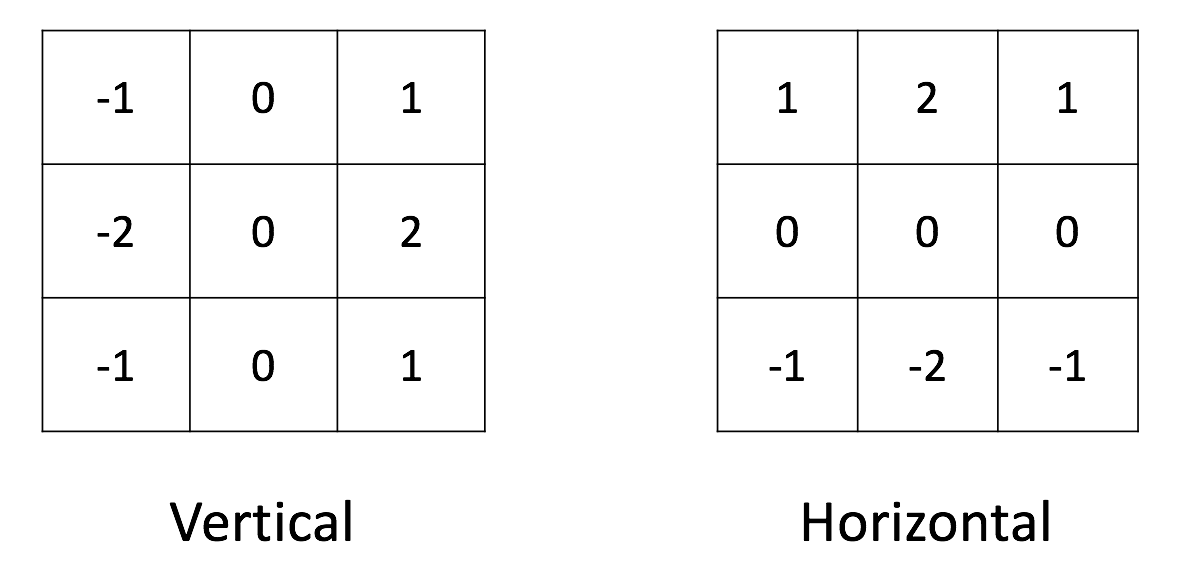
\includegraphics[width=300pt]{pic/3_2_5.png}
    \end{center}
\end{figure}
\\\\
左邊的Vertical Kernel可以偵測出垂直的線段,右邊的Horizontal Kernel可以偵測出水平的線段。待會我們會看實際的結果。
\\接下我們就來講解Canny Edge Detector又是怎麼做的。相對Sobel Operator他就複雜多了。首先我們的圖片會先移除雜訊,接著我們會找出圖片中的梯度,並且除去較不真實的結果,然後再取出有可能是邊緣的地方。雖然以上步驟看似困難,但我們都可以用OpenCV的函式輕易完成,我們先稍微看過程式碼跟結果。
\begin{figure}[htp]
    \begin{center}
        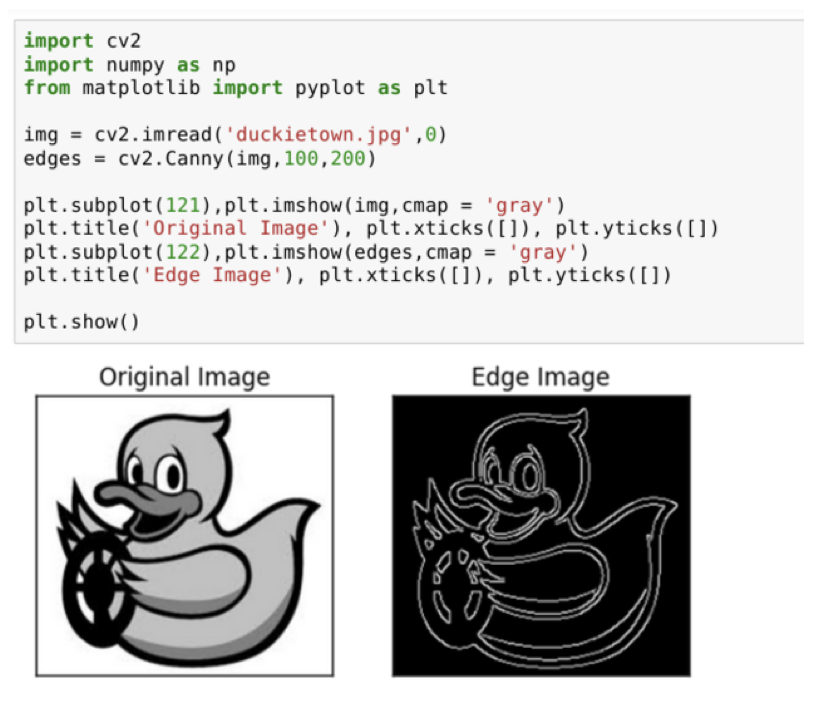
\includegraphics[width=300pt]{pic/3_2_6.png}
    \end{center}
\end{figure}
\\
實際應用
\\我們把Canny邊緣運算子套在我們要運算的圖片上面就是這個樣子。可以看到圖中我們已經把裡面的邊緣都匡起來了,也可以找到許多道路線段的痕跡。
\begin{figure}[htp]
    \begin{center}
        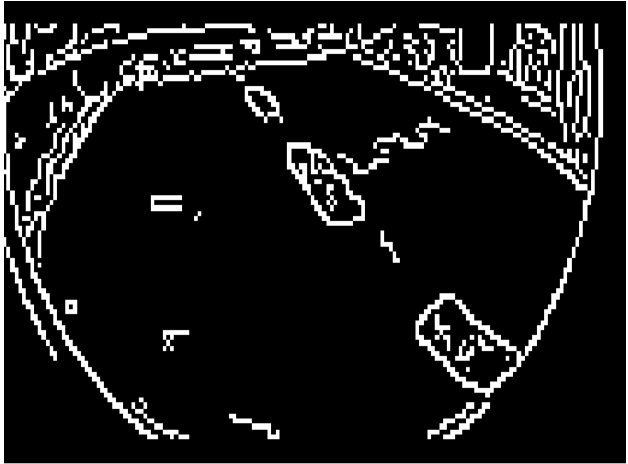
\includegraphics[width=250pt]{pic/3_2_19.png}
    \end{center}
\end{figure}
\\

\subsection{HSV Color Space \& Thresholding (HSV色彩空間與閾質判斷)}
HSV Color Space (HSV色彩空間)
在這裡我們先簡單介紹HSV色彩空間是什麼,我們可以用一個有趣的例子來介紹
\begin{figure}[htp]
    \begin{center}
        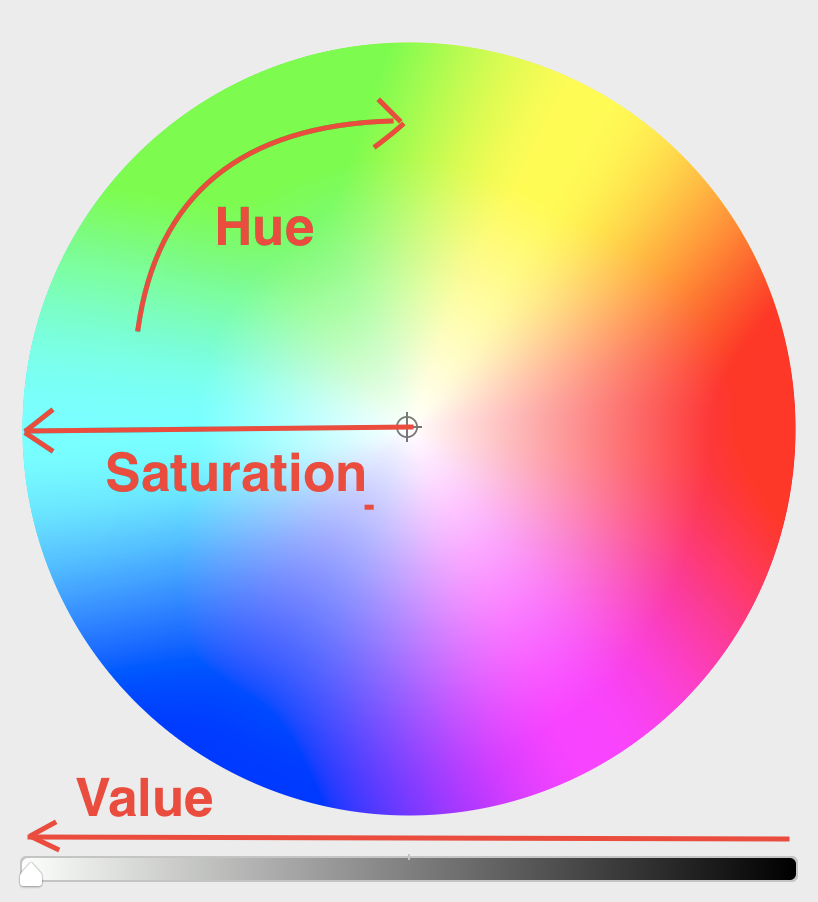
\includegraphics[width=200pt]{pic/3_2_8.png}
    \end{center}
\end{figure}
\\
這是蘋果電腦的調色盤,他就是使用HSV色彩空間調出各種顏色。HSV色彩空間其實就是另一種表示顏色的方式,就像我們平常使用的RGB。那我們可以看到圖中,”Hue”表示類似不同的色彩區域,“Saturation”則類似色彩飽和度,”Value”則類似色彩量的多寡。而每個值分別是0~255。(除了”Hue”是0~127)
\\至於為何要使用HSV色彩空間則是因為,在HSV空間裡差不多的顏色會是在連起來的區塊裡,較適合我們拿來做色彩的判斷。
\\\\HSV Thresholding (HSV閾質判斷)
如果我們要找出黃色和白色線段,就要找出圖中黃色和白色的區域。
\begin{figure}[htp]
    \begin{center}
        
\includegraphics[width=200pt]{pic/3_2_9.png}
    \end{center}
\end{figure}
\\
當該像素點位於我們需要的HSV白色/黃色的空間內,我們就把它標記起來,這就是標記後的結果。就是所謂的HSV Tresholding。

\subsection{AND邏輯閘和Hough Transform (霍夫轉換)}
最後我們將兩張圖用AND邏輯閘結合再一起
\begin{figure}[htp]
    \begin{center}
        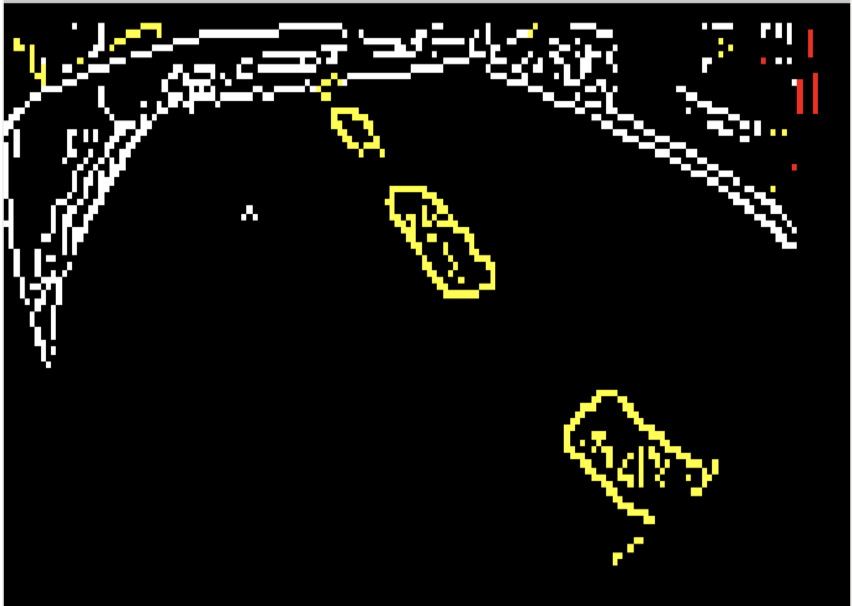
\includegraphics[width=200pt]{pic/3_2_10.png}
    \end{center}
\end{figure}
\\
在裡面我們就可以分辨出道路黃線與白線的部分。接下來我們會使用Hough Transform(霍夫轉換)找出線段的部分,因為真正的到路線會以線段的方式出現,可以幫助我們去除明顯不是道路線段的部分,也是我們之後判斷車體在哪裡的一個基準。
\\下圖中黑色就是電腦判斷為白色線段的部分,藍色為電腦判斷為黃色線斷的部分。
\begin{figure}[htp]
    \begin{center}
        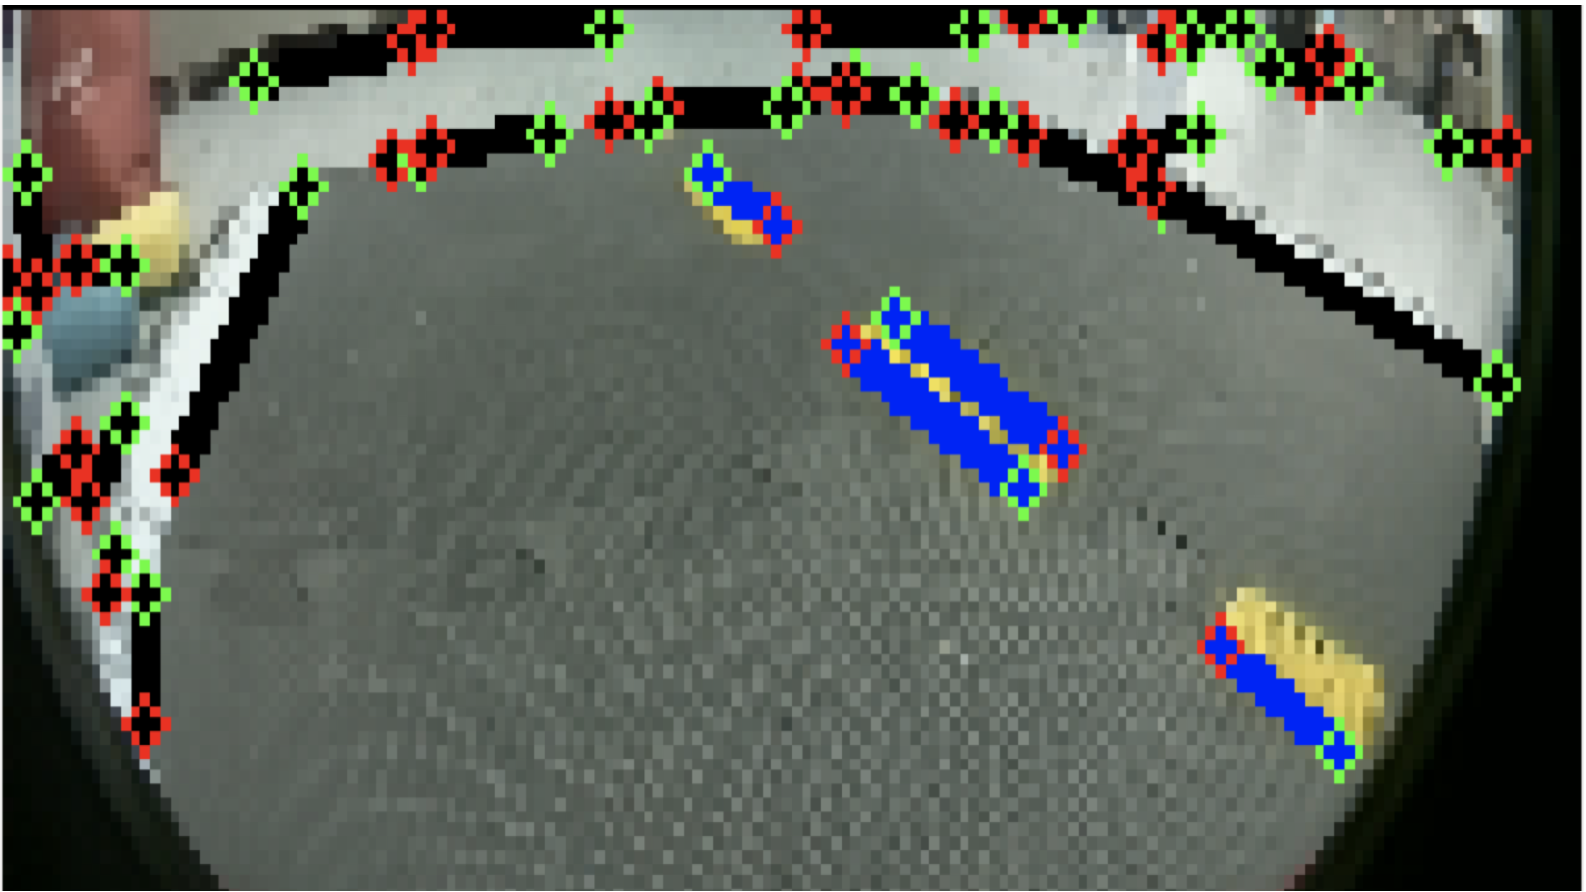
\includegraphics[width=200pt]{pic/3_2_11.png}
    \end{center}
\end{figure}
\\\\\\

\subsection{小試身手!}
接著我們就來看實際程式碼的部分囉!我們會將剛剛說的理論部分直接以程式碼實現!請大家用Jupyter Notebook開啟4-2的檔案。
\\\\縮小圖片與邊緣偵測
\\首先這部分就是簡單地縮小圖片
\begin{figure}[htp]
    \begin{center}
        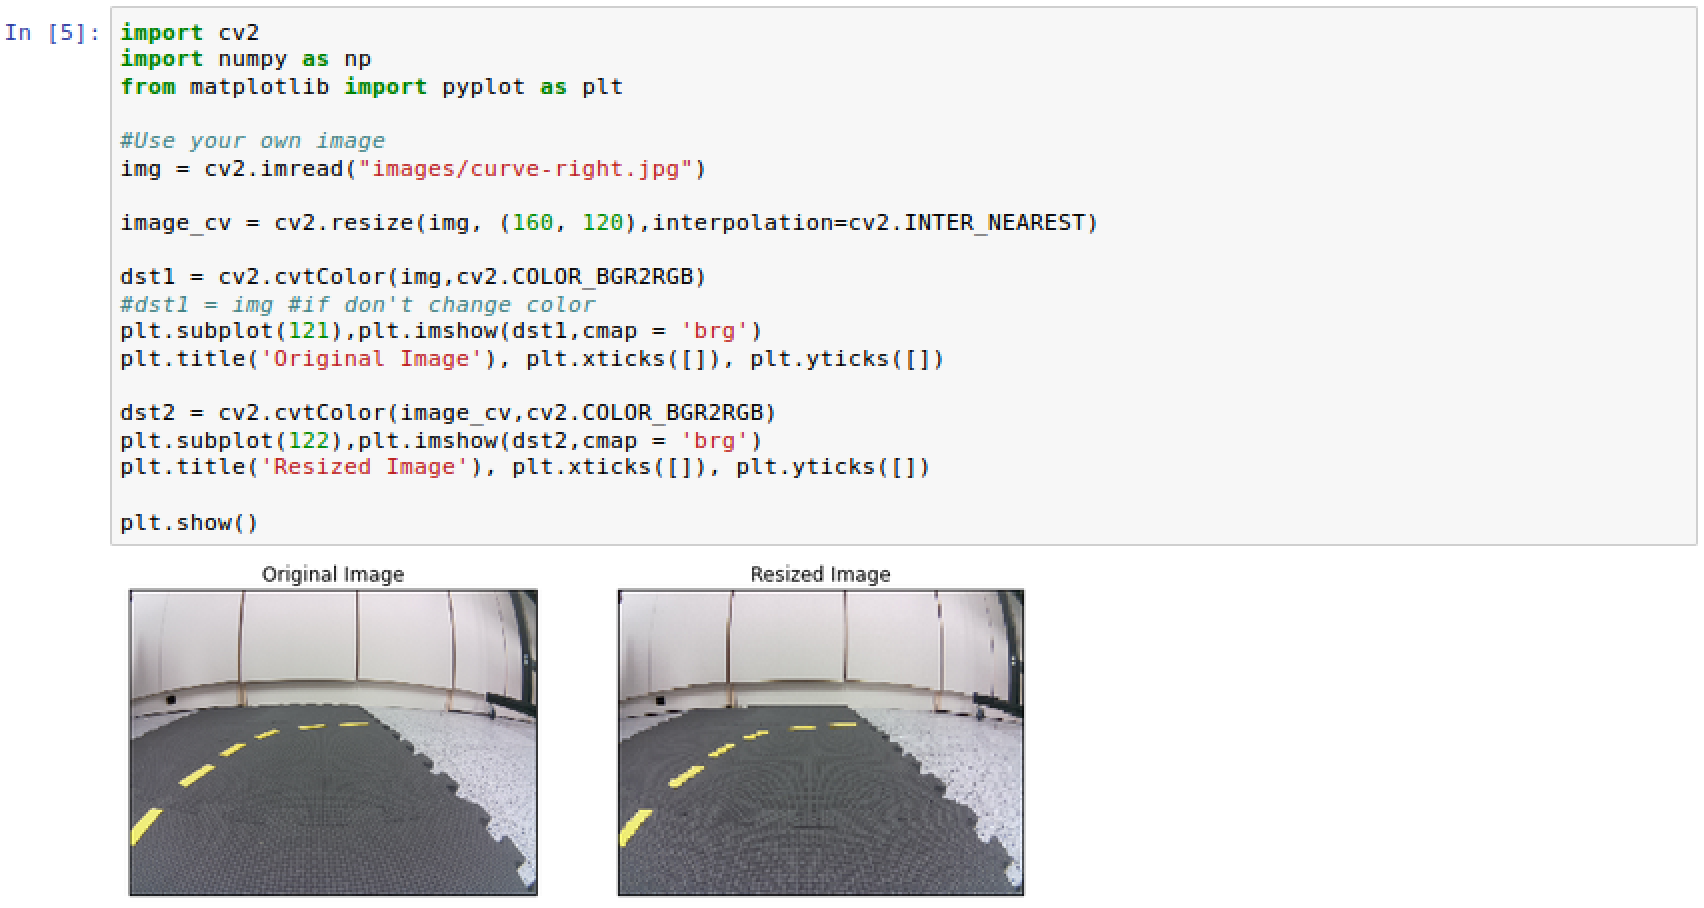
\includegraphics[width=400pt]{pic/3_2_12.png}
    \end{center}
\end{figure}
\\
以及找到圖片中的邊緣
\\這些部分雖然原理複雜,但用函式庫可以很快就完成喔!大家也可以試試Canny邊緣運算子的兩個參數,看看哪些參數的效果最好。
\begin{figure}[htp]
    \begin{center}
        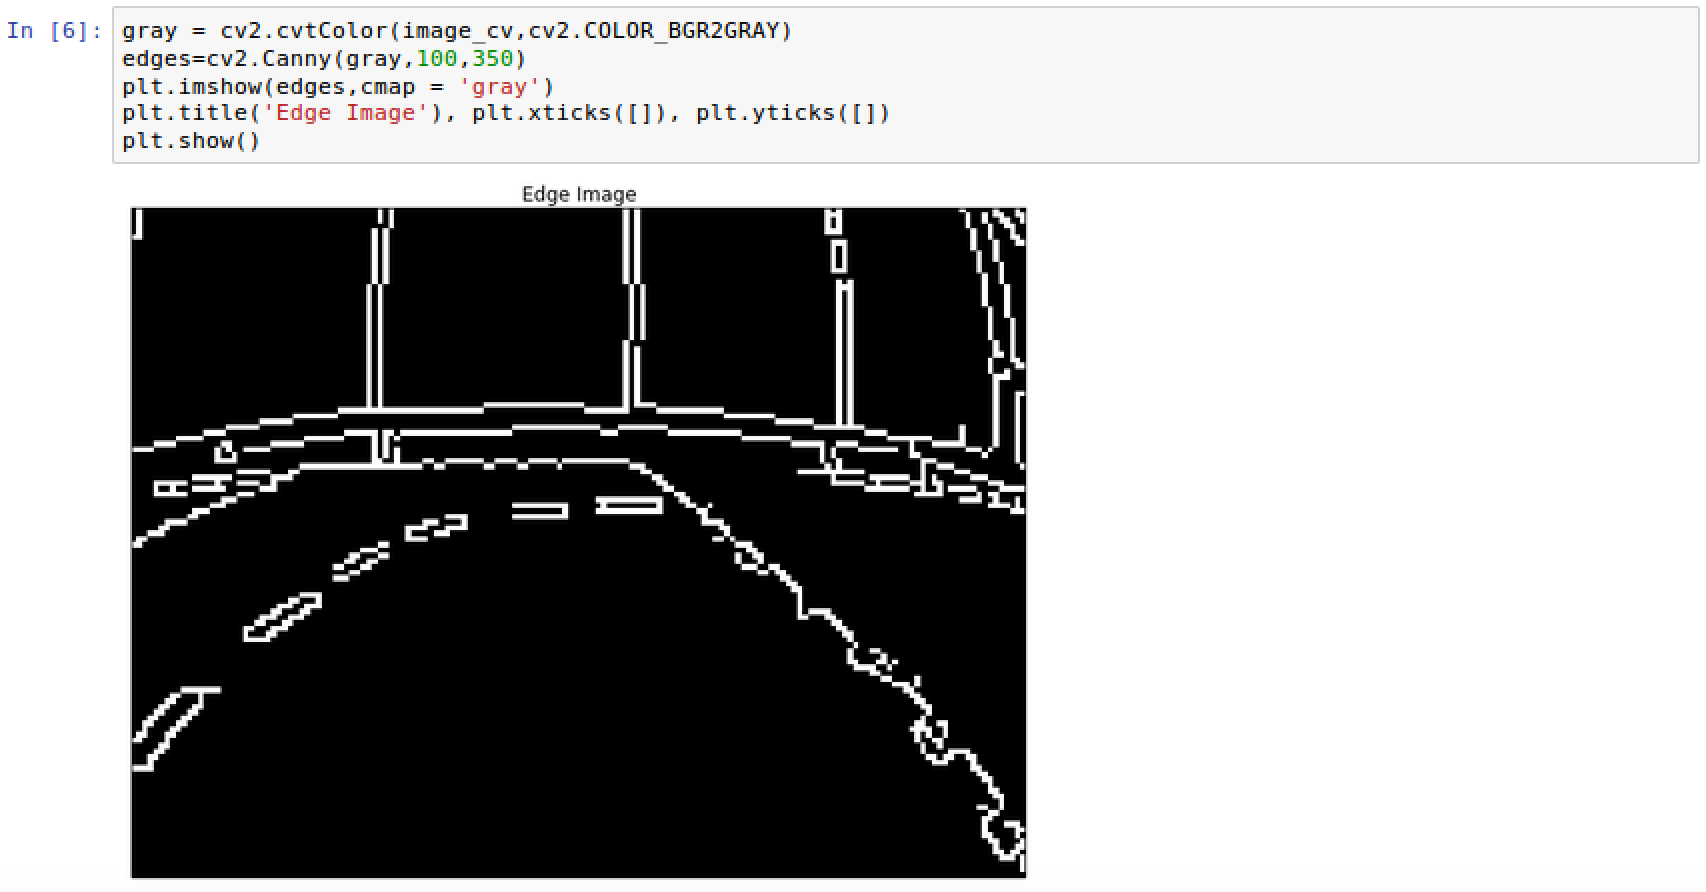
\includegraphics[width=400pt]{pic/3_2_13.png}
    \end{center}
\end{figure}
\\\\\\\\\\\\\\
HSV Thresholding (HSV閾質判斷)
\\接下來我們要做HSV閾質判斷,也就是哪邊是黃色、哪邊是白色以及紅色。在判斷之前我們要先定義”什麼是黃色、紅色、白色“
\begin{figure}[htp]
    \begin{center}
        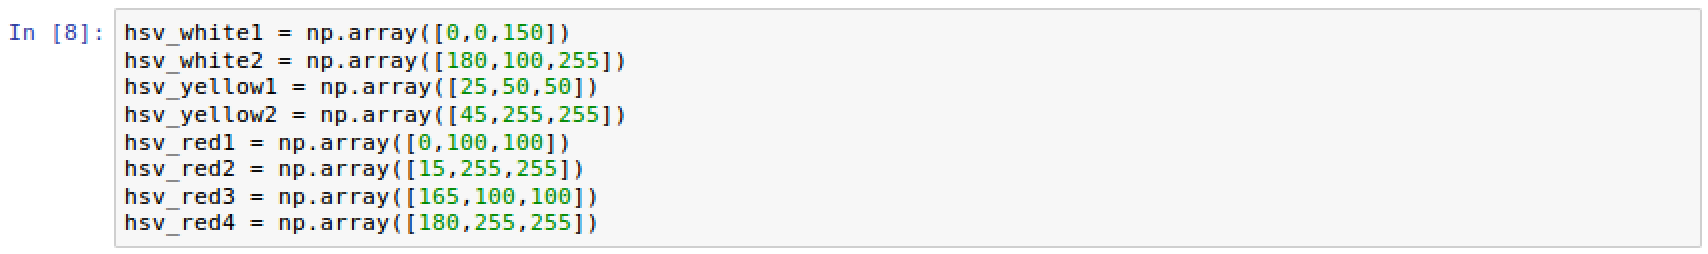
\includegraphics[width=400pt]{pic/3_2_14.png}
    \end{center}
\end{figure}
\\
大家可以看到,當我的Hue落在0到180、Saturation落在0到100、Value落在150到255時,就是白色!其他以此類推。接下來是判斷以及判斷結果展示
\begin{figure}[htp]
    \begin{center}
        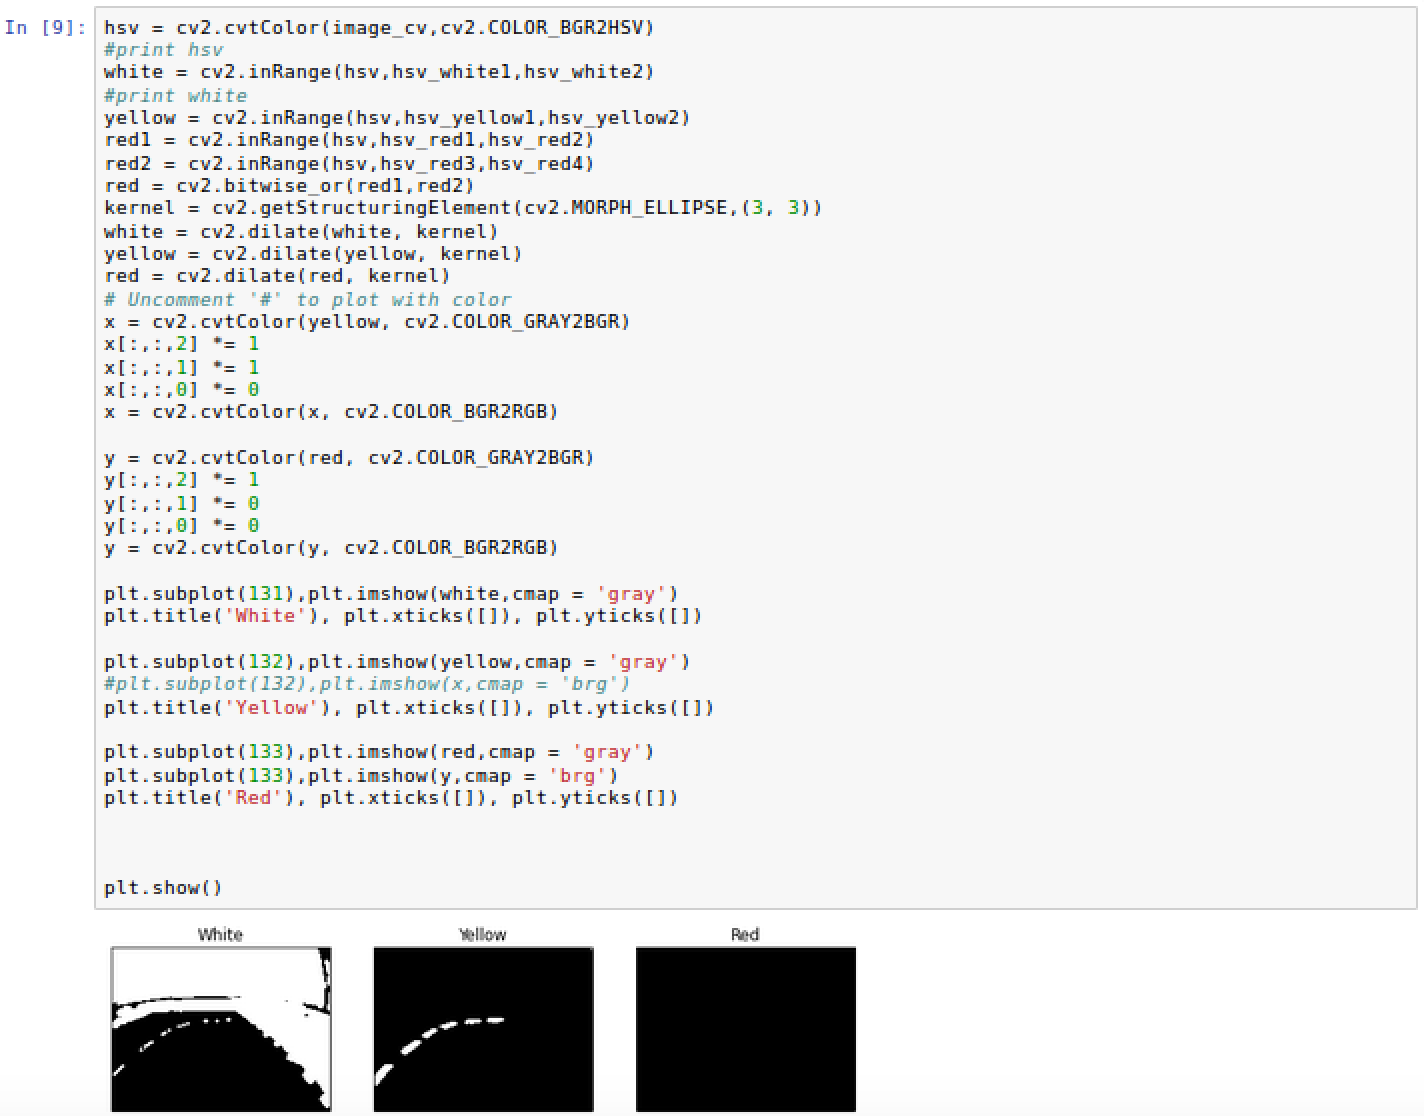
\includegraphics[width=350pt]{pic/3_2_15.png}
    \end{center}
\end{figure}
\\
\\\\\\\\\\\\\\\\\\\\\\\\\\\\\\結合邊緣偵測及HSV閾質判斷
\\接下來就要做我們所謂AND閘的部分
\begin{figure}[htp]
    \begin{center}
        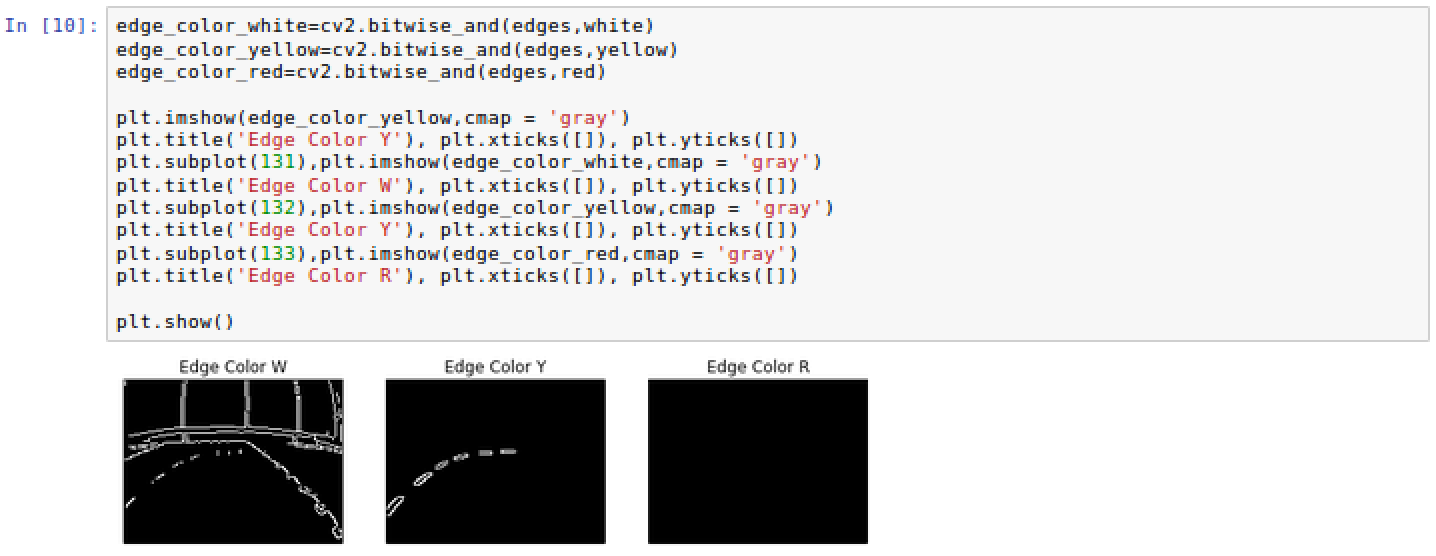
\includegraphics[width=350pt]{pic/3_2_16.png}
    \end{center}
\end{figure}
\\
找出線段
\\最後就是利用Hough Transform找出線段
\begin{figure}[htp]
    \begin{center}
        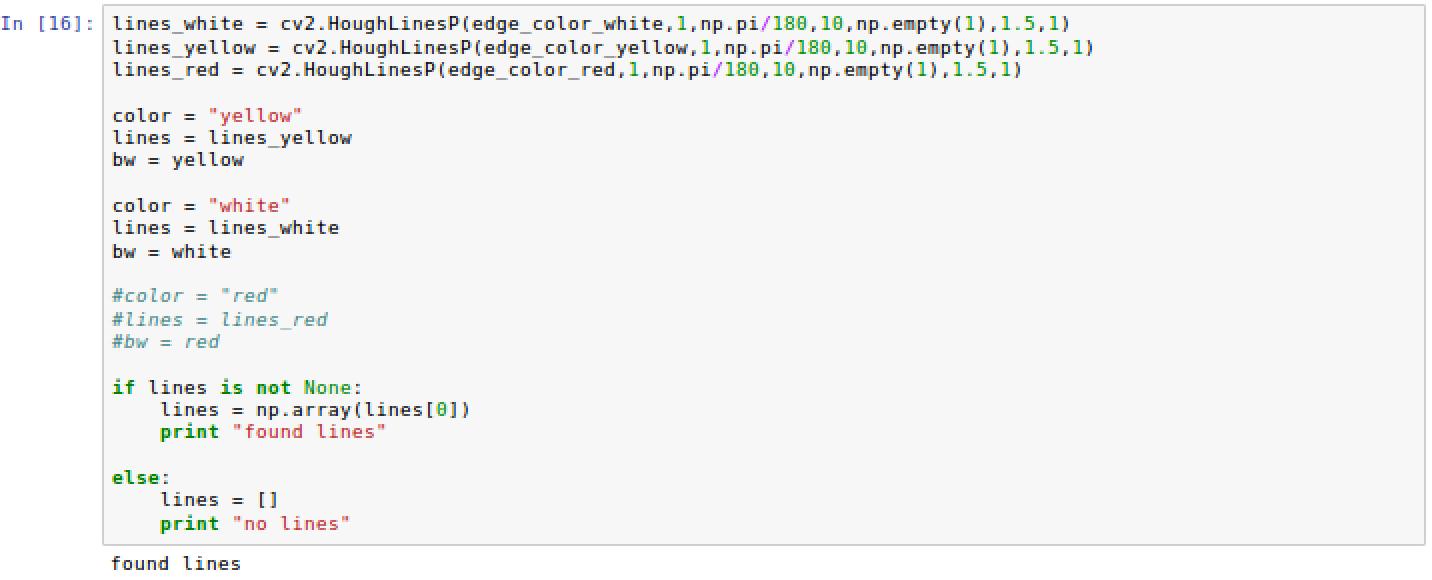
\includegraphics[width=400pt]{pic/3_2_17.png}
    \end{center}
\end{figure}
\\
\\\\\\\\\\索貝爾算子(Sobel Operator)
我們來看一下,雖然沒有用到但是也很有趣的索貝爾算子
\begin{figure}[htp]
    \begin{center}
        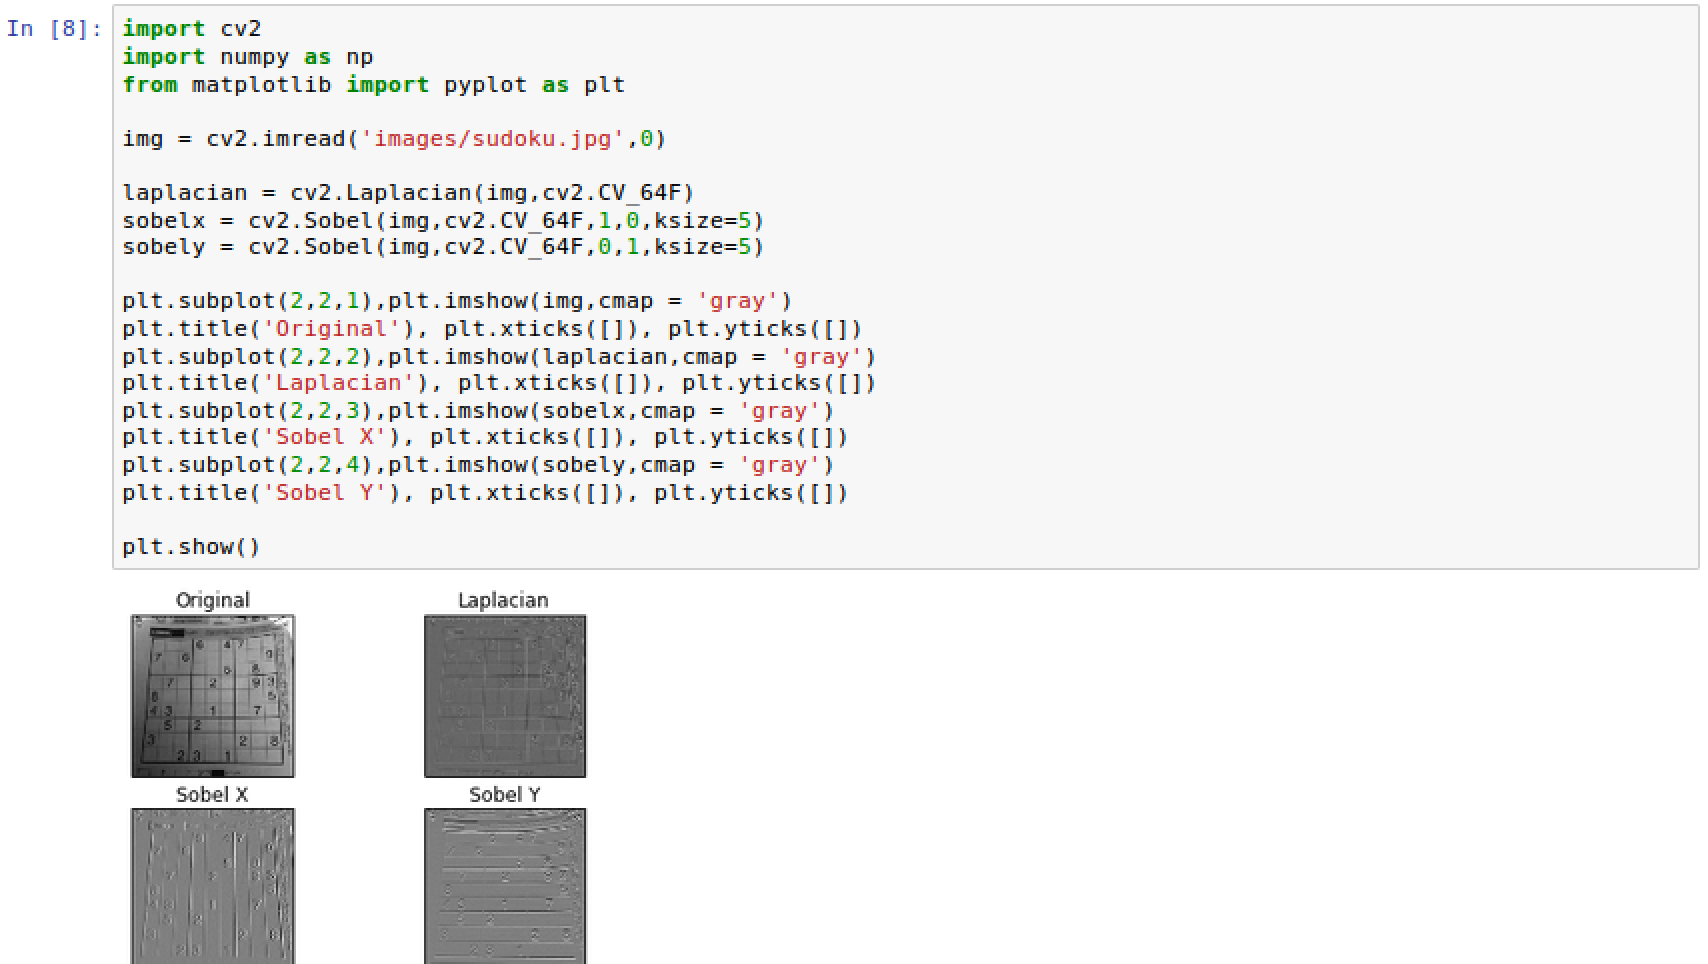
\includegraphics[width=400pt]{pic/3_2_18.png}
    \end{center}
\end{figure}
\\
我們可以看到,水平與垂直的索貝爾算子可以分別得到垂直與水平的邊緣。

\newpage
\section{Lane Filter \& 車體控制}
\subsection{Lane Filter}
Lane Filter較難找到一個適合的中文翻譯,不過基本上Lane Filter在做的就是判斷車體在道路中相對的位置。我們接下來就來解釋他怎麼運作的吧!
\\這裡我們要分成四個部分來解釋,首先想知道車體在道路中的相對位置,就要知道我們怎麼表示車子的位置。接下來我們會利用一種”投票”的機制來決定車子的位置。最後我們會用貝式濾波器來讓產生這個預測與執行的控制迴圈。(貝式率波器將不會出現在本書,有興趣可上交大OCW觀看)
\\\\State (車子狀態)
State(狀態)可以用來描述一系列機器人與環境可以對未來造成影響的部分。聽起來很複雜,但我們這裡先告訴大家描述車體的位置的方式。請看下圖
\begin{figure}[htp]
    \begin{center}
        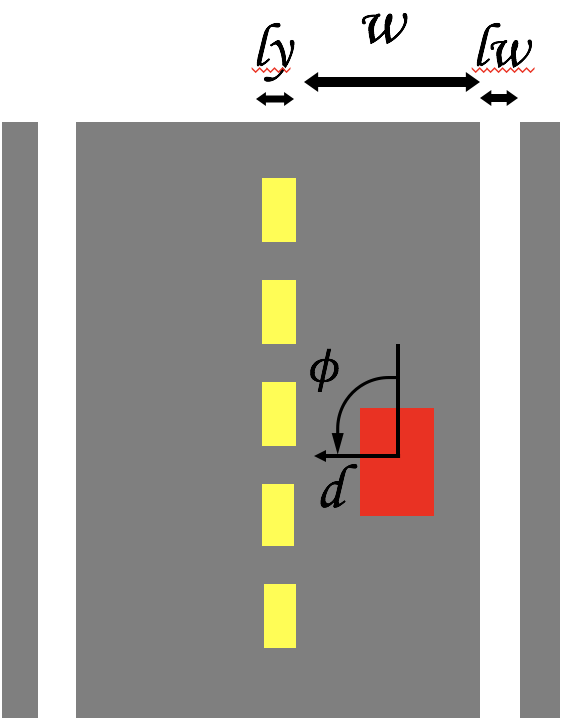
\includegraphics[width=150pt]{pic/3_3_1.png}
    \end{center}
\end{figure}
\\
我們可以看到,這裡使用兩個變數描述車體的位置。d表示車體與道路中線的距離,而𝝓則表示該位置與垂直的相對角度。
\\\\Measure Model (量測模型)
接下來我們要做的就是剛剛有提到的“投票”機制,我們會利用上一章所提到的,產生的線段。利用這些線段進行投票,以描述出車體與道路間的相對位置。我們會把各線段利用剛剛的表示方法拿來做計算,也就是會有這樣的一個轉換
\begin{figure}[htp]
    \begin{center}
        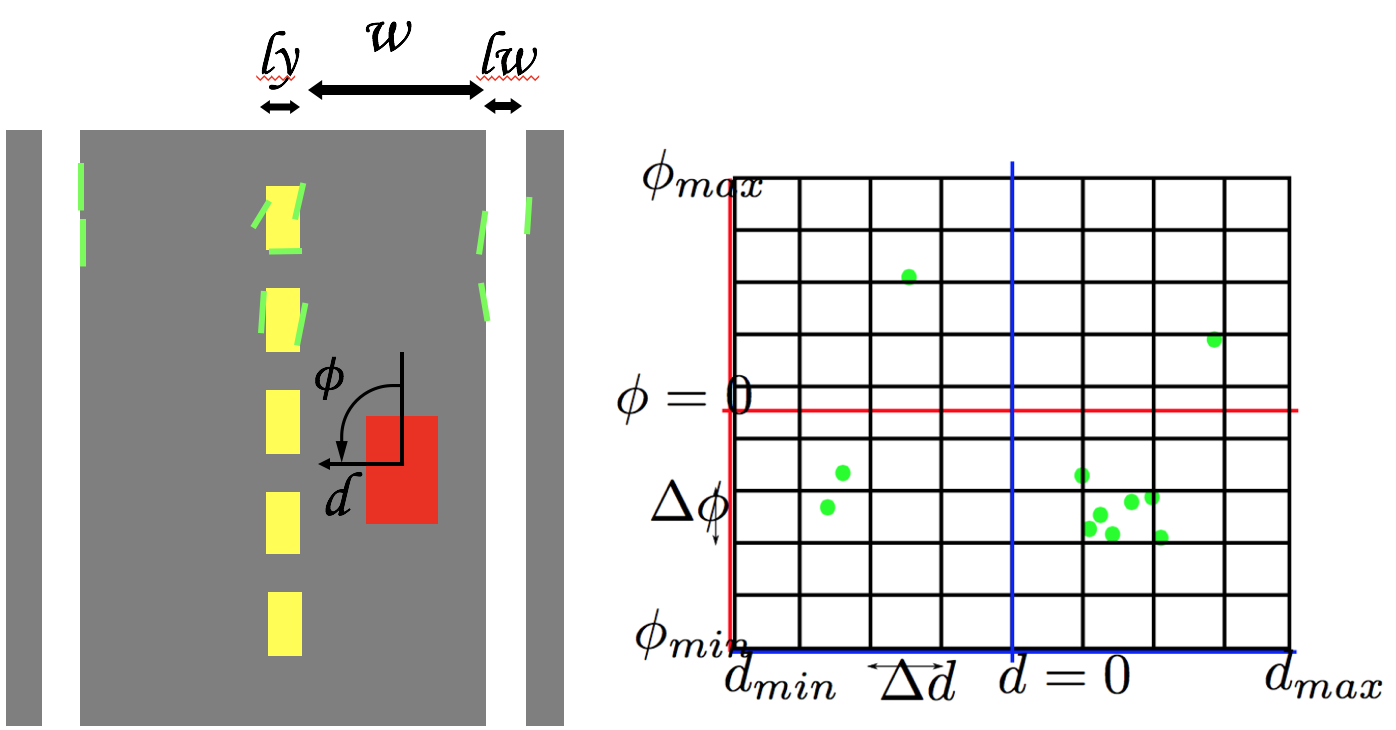
\includegraphics[width=400pt]{pic/3_3_2.png}
    \end{center}
\end{figure}
\\
將這些得到的線段位置拿去做一個“投票”的動作,就可以決定出車子的位置。
\\\\\\\\\\\\\\\\
\subsection{Car Command (車體控制)}
最後我們若得到車子的相對位置,就可以對他進行相對應的控制。

\subsection{小試身手!}
說了這麼多,我們不如直接來試試看吧!在我們開始之前有一些部分要進行設定,為了等等的車體控制的部分。
\\首先我們需要跟改筆電這裡的hostname,請更改robotvision至你想要的hostname
\\\$ duckietop: sudo vim /etc/hostname 
\begin{figure}[htp]
    \begin{center}
        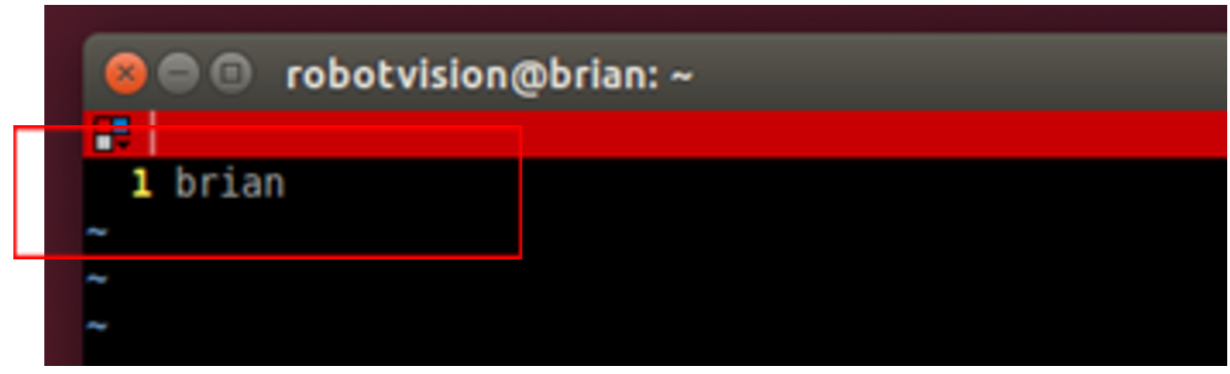
\includegraphics[width=400pt]{pic/3_3_3.png}
    \end{center}
\end{figure}
\\
增加”127.0.1.1 hostname hostname.local”
\\\$ duckietop: sudo vim /etc/hosts
\begin{figure}[htp]
    \begin{center}
        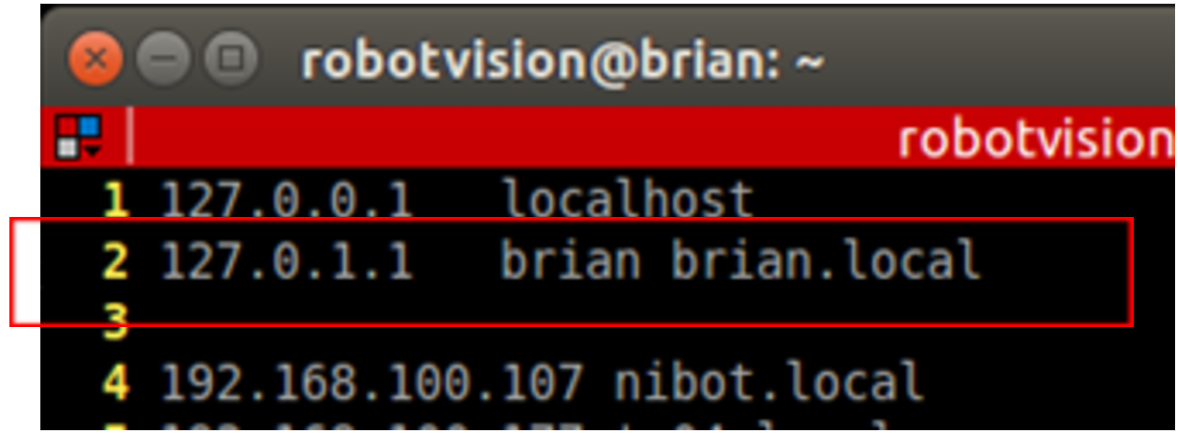
\includegraphics[width=400pt]{pic/3_3_4.png}
    \end{center}
\end{figure}
\\
\\\\\\\\連線進車子,將筆電的IP位址加進去
\\\$ duckiebot: sudo vim /etc/hosts 
\begin{figure}[htp]
    \begin{center}
        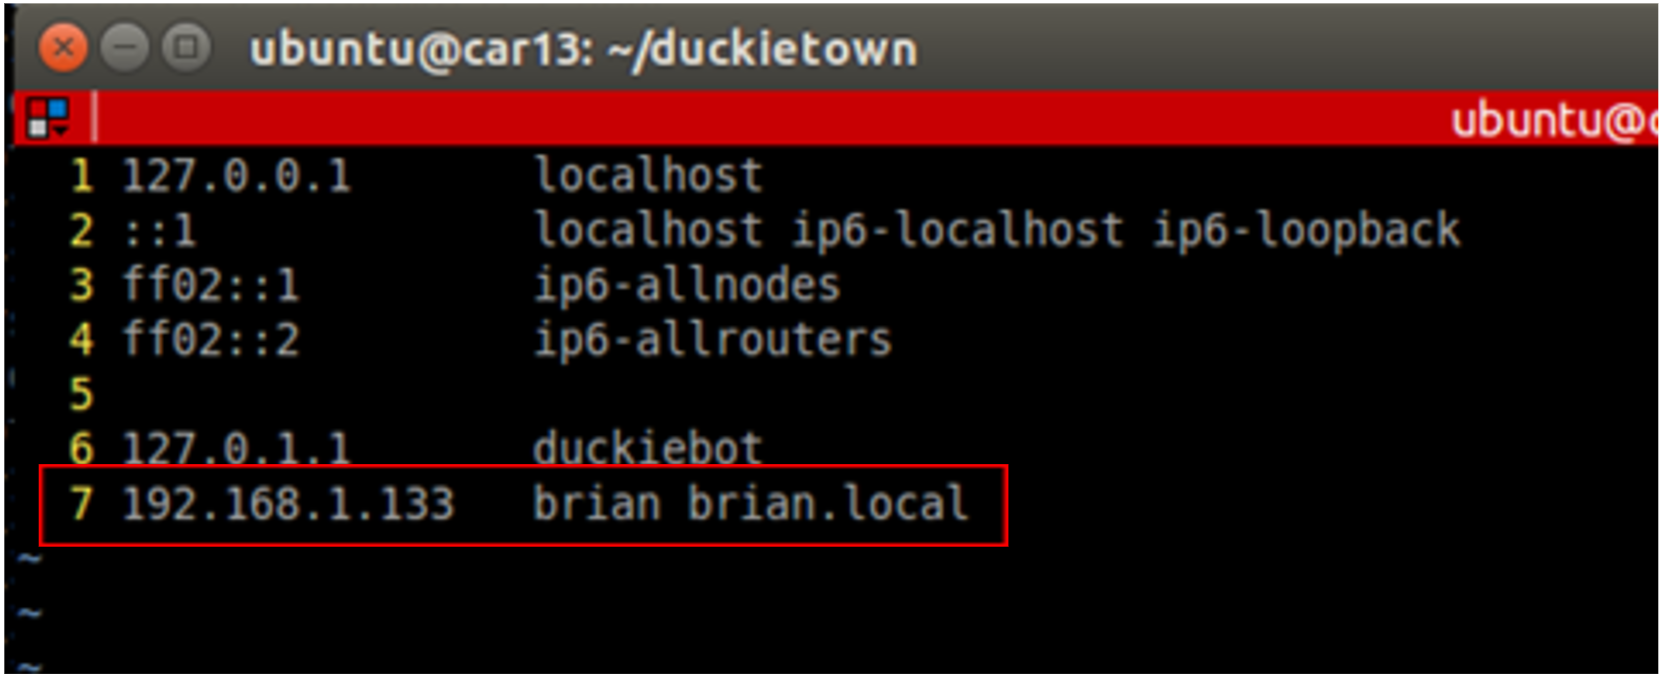
\includegraphics[width=400pt]{pic/3_3_5.png}
    \end{center}
\end{figure}
\\
接下來我們需要把車子上的launch打開,已接受筆電傳的訊息。記得將car13改成你的車子的名稱
\\\$ duckiebot: cd ~/duckietown
\\\$ duckiebot: source environment.sh
\\\$ duckiebot: source set\_ros\_master.sh
\\\$ duckiebot: roslaunch duckietown\_nctu\_wama joystick\_jupyter.launch veh:=car13
\\\\最後我們要開啟Jupyter Notebook來控制車子。
\\\$ duckietop: source ~/duckietown/catkin\_ws/devel/setup.bash
\\\$ duckietop: source ~/duckietown/set\_ros\_master.sh car13
\\\$ duckietop: cd ~/duckietown/tutorials/summer2017\_nctu
\\\$ duckietop: jupyter notebook 4-3.lane\_filter\_drive.ipynb





\end{document}

















